
%  Created by Colin Williams on 2012-01-06.
%  Copyright (c) 2012 __MyCompanyName__. All rights reserved.
%
\documentclass[]{article}

% Use utf-8 encoding for foreign characters
\usepackage[utf8]{inputenc}

% Setup for fullpage use
\usepackage{fullpage}

% Uncomment some of the following if you use the features
%
% Running Headers and footers
%\usepackage{fancyhdr}

% Multipart figures
%\usepackage{subfigure}

% More symbols
%\usepackage{amsmath}
%\usepackage{amssymb}
%\usepackage{latexsym}

% Surround parts of graphics with box
\usepackage{boxedminipage}

% Package for including code in the document
\usepackage{listings}

% If you want to generate a toc for each chapter (use with book)
\usepackage{minitoc}

% This is now the recommended way for checking for PDFLaTeX:
\usepackage{ifpdf}
\usepackage{comment}

%\newif\ifpdf
%\ifx\pdfoutput\undefined
%\pdffalse % we are not running PDFLaTeX
%\else
%\pdfoutput=1 % we are running PDFLaTeX
%\pdftrue
%\fi


\usepackage{array}
\usepackage{url}
\usepackage{listings}
\usepackage{color}
\usepackage{amsmath}
\usepackage{mathtools}

\definecolor{dkgreen}{rgb}{0,0.6,0}
\definecolor{gray}{rgb}{0.5,0.5,0.5}
\definecolor{mauve}{rgb}{0.58,0,0.82}

\lstset{
  language=Java,
  tabsize=4,
  showstringspaces=false,
  basicstyle=\tt,
  numberstyle=\tiny\color{gray},      % line number style
  keywordstyle=\color{blue},          % keyword style
  commentstyle=\color{dkgreen},       % comment style
  stringstyle=\color{mauve},          % string literal style
}

\ifpdf
\usepackage[pdftex]{graphicx}
\else
\usepackage{graphicx}
\fi
\title{Negotiation User Guide}
\author{T. Baarslag, W. Pasman, K. Hindriks, D. Tykhonov, W. Visser, M. Hendrikx, D. Feirstein}

\date{\today}

% Alter some LaTeX defaults for better treatment of figures:
    % See p.105 of "TeX Unbound" for suggested values.
    % See pp. 199-200 of Lamport's "LaTeX" book for details.
    %   General parameters, for ALL pages:
    \renewcommand{\topfraction}{0.9}	% max fraction of floats at top
    \renewcommand{\bottomfraction}{0.8}	% max fraction of floats at bottom
    %   Parameters for TEXT pages (not float pages):
    \setcounter{topnumber}{2}
    \setcounter{bottomnumber}{2}
    \setcounter{totalnumber}{4}     % 2 may work better
    \setcounter{dbltopnumber}{2}    % for 2-column pages
    \renewcommand{\dbltopfraction}{0.9}	% fit big float above 2-col. text
    \renewcommand{\textfraction}{0.07}	% allow minimal text w. figs
    %   Parameters for FLOAT pages (not text pages):
    \renewcommand{\floatpagefraction}{0.7}	% require fuller float pages
	% N.B.: floatpagefraction MUST be less than topfraction !!
    \renewcommand{\dblfloatpagefraction}{0.7}	% require fuller float pages

	% remember to use [htp] or [htpb] for placement
	
\begin{document}

\ifpdf
\DeclareGraphicsExtensions{.pdf, .jpg, .tif}
\else
\DeclareGraphicsExtensions{.eps, .jpg}
\fi

\maketitle

\newcommand\Genius{{\sc Genius}}

\abstract{\noindent \Genius \cite{Genius}~is a negotiation environment that implements an open architecture for heterogeneous negotiating agents. \Genius~can be used to implement, or simulate, real life negotiations. This document describes how you can install the environment, work with the provided scenarios and negotiation agents, and write, compile, and run an agent yourself.}

\pagebreak
\tableofcontents

\pagebreak


%=========================================================================================
\section{Theory Crash Course}
This section provides a crash course on some essential theory needed to understand the negotiation system. Furthermore, it provides an overview of the features of a negotiation implemented in \Genius.

\subsection{Negotiation Objects}
Agents participating in a negotiation interact in a scenario. A scenario specifies the possible bids and their preference for both agents. A scenario consists of a domain (also called the outcome space) and a number of utility spaces (also called preference profiles) -- one for each party/agent in the negotiation. Figure~\ref{Fig:overviewStructures} provides an overview of the relation between the domain and the utility space of an agent.

\begin{figure}[htb]
	\centering
	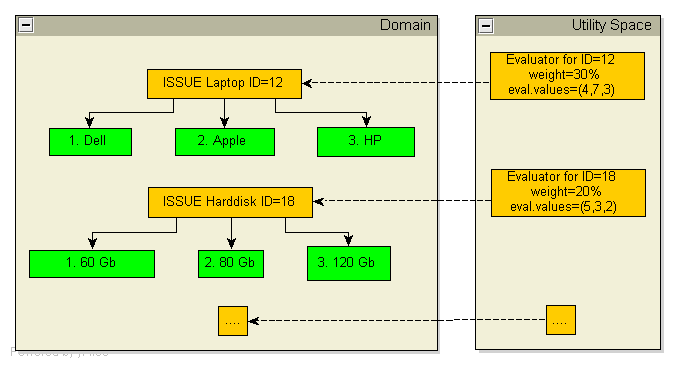
\includegraphics[width=0.8\textwidth]{media/datastructures.png}
	\caption{Overview of the data structures and relations.}\label{Fig:overviewStructures}
\end{figure}

The \textit{Domain} describes which issues are the subject of the negotiation and which values an issue can attain. A domain contains $n$ issues: $D=(I_1,\ldots,I_n)$. Each issue $i$ consists of $k$ values: $I_i=(v^i_1,\ldots,v^i_k)$.  Combining these concepts, an agent can formulate a \textit{Bid}: a mapping from each issue to a chosen value (denoted by $c$), $b=(v^i_{c},\ldots,v^n_{c})$. 

To give an example, in the laptop domain the issues are ``laptop'', ``harddisk'' and ``monitor''. In this domain the issues can only attain discrete values, e.g. the ``harddisk'' issue can only have the values ``60 Gb'', ``80 Gb'' and ``120 Gb''. These issues are all instance of \textit{IssueDiscrete}. A valid bid in the laptop domain is a Dell laptop with 80 Gb and a 17' inch monitor.

The \textit{Utility Space} specifies the preferences of the bids for an agent using an evaluator. The evaluator of an issue maps the evaluation of an issue value -- which is specified in the preference profile -- to a utility for that issue. The evaluator also specifies the importance of the issue relative to the other issues in the form of a weight. The weights of all issues sum up to 1.0 to simplify calculating the utility of a bid. To illustrate, the ``harddisk'' issue is of the type \textit{IssueDiscrete}, and therefore its evaluator is of the type \textit{EvaluatorDiscrete}.

In general, given the set of all bids, there are a small subset of bids which are more preferred as outcomes by both agents. Identifying these special bids may lead to a better agreement for both parties. We discuss the optimality of a bid in the next section.

\subsection{Optimality of a Bid}
%Before discussing the optimality of a bid, we first need to formalize the concept of a bid. 
%A bid is a set of chosen values $v_1, \ldots, v_n$  for each of the $N$ issues. Each of these values has been assigned an evaluation value $\text{eval}(v_i)$ in the utility space. The utility is the weighted sum of the scaled evaluation values.
%A bid is a set of values, one chosen for each issue $n$ in the domain. (the subscript $c$ denotes the chosen value for issue $i$).
Each value of a bid is assigned an evaluation value $\text{eval}(v^n_{c})$ in the utility space. The utility is the weighted sum of the scaled evaluation values.

\begin{equation}
	U(v^i_{c},\ldots,v^n_{c}) = \sum_{i=1}^{n} w_i \dfrac{\text{eval}(v^i_{c})}{\text{max}(\text{eval}(I_i))}
	\label{eqn:Utility}
\end{equation}

%\begin{equation}
%	U(v_1, \ldots, v_n) = \sum_{i=1}^{N} w_i \dfrac{\text{eval}(v_i)}{\text{max}(\text{eval}(v_i))}
%	\label{eqn:Utility}
%\end{equation}
\pagebreak

For a single agent, the optimal bid is of maximum utility for the agent. Often this bid has a low utility for the opponent, and therefore the chance of agreement is low. A more general notion of optimality of a negotiation involves the utility of both agents.
\begin{figure}[htb]
	\centering
	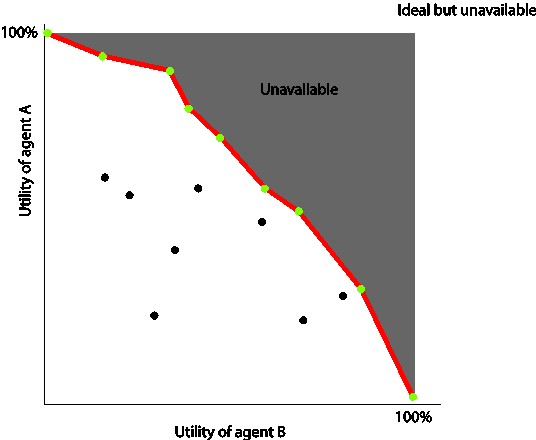
\includegraphics[width=0.37\textwidth]{media/image5.png}
\caption{A point indicates the utility for both agents of a bid. The red line is the Pareto optimal frontier.}\label{Fig:utility plot}
\end{figure}

There are multiple ways to define a more global ``optimum''. One approach to optimality is that a bid is not optimal for both parties if there is another bid that has the higher utility for one party, and at least equal utility for the other party. Thus, only bids in Figure~\ref{Fig:utility plot} for which there is no other bid at the top right is optimal. This type of optimality is called Pareto optimality and forms an important concept in automated negotiation. The collection of Pareto optimal bids is called the Pareto optimal frontier.

A major challenge in a negotiation is that agents can hide their preferences. This entails that an agent does not know which bid the opponent prefers given a set of bids. This problem can be partly resolved by building an \textit{opponent model} of the opponent's preferences by analyzing the negotiation trace. Each turn the agent can now offer the best bid for the opponent given a set of similar preferred bids. \Genius  provides a number of components that can estimate an opponent model.

\subsection{Negotiation Protocol}
The negotiation protocol determines the overall order of actions during a negotiation. Agents are obliged to stick to this protocol, as deviations from the protocol are caught and penalized. This section discusses the details of the bilateral alternating offers protocol used in \Genius.

In the bilateral alternating offers protocol two parties -- agent $A$ and agent $B$ -- take turns. Agent $A$ starts the negotiation. Each turn an agent presents one of the three possible actions:

\begin{center}
\begin{tabular}{cm{0.6\textwidth}}
\hline
\textsc{Accept} & This action indicates that agent accepts the opponent's last bid.\\
\hline
\textsc{Offer} & This action represents the bid made by an agent.\\
\hline
\textsc{EndNegotiation} & This action indicates that the agent terminates the negotiation.\\
\hline
\end{tabular}
\end{center}

When it is an agent's turn, it is informed about the opponent's action. Based on the opponent's action the agent comes up with an action, which it presents to the opponent. Sequentially, the opponent presents a counter action. This process goes on until the negotiation finishes in one of the following ways:
\begin{itemize}
	\item An agent accepts the opponent's offer using the action \textsc{Accept}. The utility of the opponent's last bid is determined for both agents according to their preference profiles. The opponent is informed of acceptance via the \textit{ReceiveMessage} method.
	\item The action returned by an agent is \textsc{EndNegotiation}. In this case the score of both agents is set to their reservation value.
	\item Finally, if an agent does not follow the protocol -- for instance by sending an action that is not one of the above or by crashing -- the agent's utility is set to its reservation value, whereas the opponent is awarded the utility of the last offer.
\end{itemize}
 
\subsection{Reservation Value}
A reservation value is a real-valued constant that sets a threshold below which a rational agent should not accept any offers. Intuitively, a reservation value is the utility associated with the Best Alternative to a Negotiated Agreement (BATNA).

A reservation value is the utility that an agent will obtain if no agreement is realized in a negotiation session. This can happen either if an agent leaves the negotiation, or by not reaching an agreement before the deadline. In other words: either the negotiating parties agree on an outcome $\omega$, and both agents receive the associated utility of $\omega$, or no agreement is reached, in which case both agents receive their reservation value instead. Reservation values typically differ for each negotiation agent. In case no reservation value is set in a profile, it is assumed to be 0.


\subsection{Time Pressure}
A negotiation lasts a predefined time in seconds, or alternatively rounds. In \Genius~the time line is \emph{normalized}, i.e.: time $t \in [0, 1]$, where $t = 0$ represents the start of the negotiation and $t = 1$ represents the deadline. Notice that manipulation of the remaining time can be a factor influencing the outcome.

There is an important difference between a time-based and rounds-based protocol. In a time-based protocol the computational cost of an agent should be taken into account as it directly influences the amount of bids which can be made. In contrast, for a rounds-based negotiation the time can be thought of as paused within a round; therefore computational cost does not play a role.

Apart from a deadline, a scenario may also feature \emph{discount factors}. Discount factors decrease the utility of the bids under negotiation as time passes. While time is shared between both agents, the discount generally differs per agent. The implementation of discount factors is as follows: let $d$ in $[0, 1]$ be the discount factor that is specified in the preference profile of an agent; let $t$ in $[0, 1]$ be the current normalized time, as defined by the timeline; we compute the discounted utility $U_D^t$ of an outcome $\omega$ from the undiscounted utility function $U$ as follows:
\begin{eqnarray}
U_D^t(\omega) = U(\omega) \cdot d^t
\end{eqnarray}
If $d = 1$, the utility is not affected by time, and such a scenario is considered to be undiscounted, while if $d$ is very small there is high pressure on the agents to reach an agreement. Note that discount factors are part of the preference profiles and therefore different agents may have a different discount factor.

If a discount factor is present, reservation values will be discounted in exactly the same way as the utility of any other outcome. It is worth noting that, by having a discounted reservation value, it may be rational for an agent to end the negotiation early and thereby default to the reservation value.
 
 
%=========================================================================================
\section{Running the Environment}
The negotiation environment has been tested extensively. It should run on any machine running Java 6 or higher, including Windows, OSX, Solaris and Linux distributions. Under Ubuntu the jar file should be launched from the terminal to avoid problems with finding the repository files. Please report any bugs found to \url{negotiation@ii.tudelft.nl}.

To install the environment, the file \texttt{Genius\_release.zip} can be downloaded. Unzip the file at a convenient location on your machine. This will result in a package called ``genius" which contains the following files:

\begin{itemize}
	\item a \texttt{doc} folder, containing \texttt{userguide.pdf} which is this document.
	\item \texttt{negosimulator.jar}, the negotiation simulator;
	\item a \texttt{tutorials} folder, containing various quick-start tutorials.
	\item a few \texttt{...package} folders, containing ready-to-compile agents and components.
	\item  a \texttt{javadoc} folder, containing the complete JavaDoc documentation of Genius.
	
\end{itemize}

When you run the negosimulator (by double-clicking the application or using open with and then selecting Java), progress messages and error messages are printed mainly to the standard output. On Mac OSX you can view these messages by opening the console window (double-click on Systemdisk/Applications/Utilities/Console.app). On Windows this is not directly possible. Console output can be read only if you start the application from the console window by hand, as follows. Go to the directory with the negosimulator and enter
\texttt{java -jar negosimulator.jar}.
This will start the simulator, and all messages will appear in the console window. You may see some errors and warnings that are non-critical.

Note that some agents and scenarios require more memory than allocated by default to Java. This problem can be resolved by using the Xmx and Xms parameters when launching the executable jar, for example \texttt{java -Xmx1536M -Xms1536M -jar negosimulator.jar}.


%=========================================================================================
\section{Scenario Creation}
A negotiation can be modeled in \Genius~by creating a scenario. A scenario consists of a domain specifying the possible bids and a set of preference profiles corresponding to the preferences of the bids in the domain. This section discusses how to create a domain and a preference profile.

\subsection{Basic GUI Components}
Start \Genius~by following the instructions in the previous section. After starting the simulator a screen similar to Figure~\ref{Fig:negosimulator start} is shown. This screen is divided in three portions:

\begin{itemize}
	\item The \textbf{Menubar} allows us to start a new negotiation.
	\item The \textbf{Components Window} shows all available scenarios, agents, and BOA components.
	\item The \textbf{Status Window} shows the negotiation status or selected domain/preference profile.
\end{itemize}

\begin{figure}[htb]
	\centering
	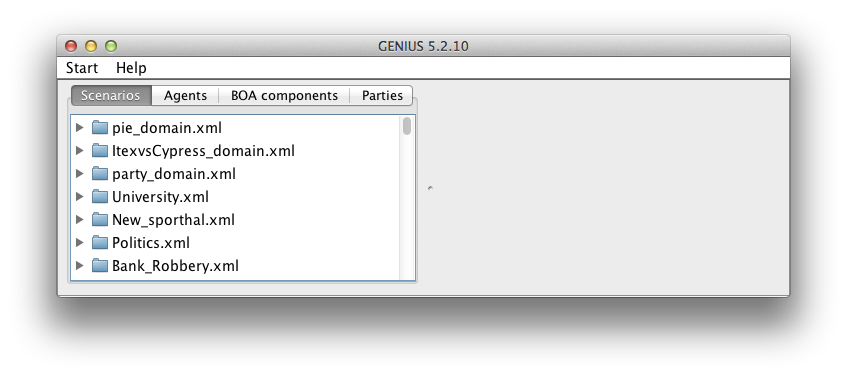
\includegraphics[width=0.6\textwidth]{media/start.png}
\caption{The negosimulator right after start-up. The left half is the components panel, the right half the status panel.}\label{Fig:negosimulator start}
\end{figure}

\subsection{Creating a Domain}
By right clicking on the list of available scenarios in the Components Window a popup menu with the option to create a new domain is shown. After clicking this option it is requested how the domain should be called. Next the domain is automatically created and a window similar to Figure~\ref{Fig:newdomain} is shown. Initially, a domain contains zero issues. We can simply add an issue by pressing the ``Add issue'' button. This results in the opening of a dialog similar to Figure~\ref{fig:createIssueD}.

\begin{figure}[htb]
	\centering
	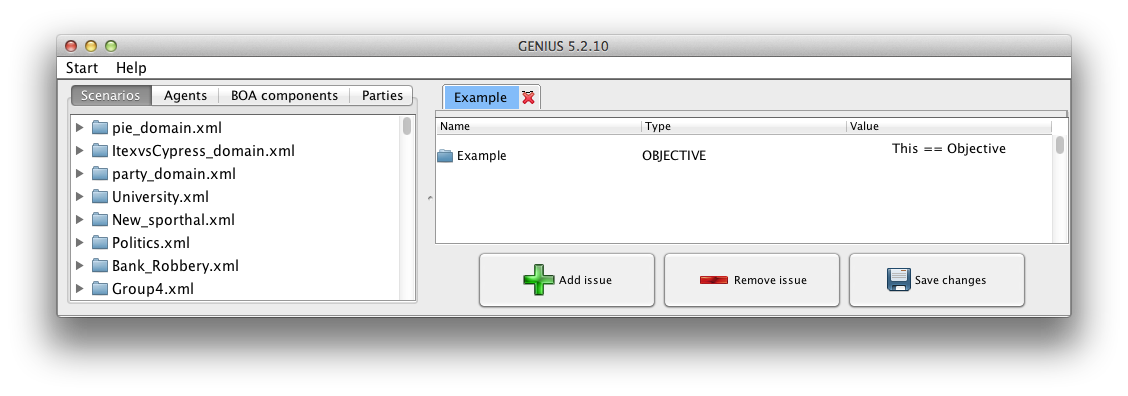
\includegraphics[width=0.9\textwidth]{media/exampledomain.png}
\caption{The negosimulator after creating a new Example domain.}\label{Fig:newdomain}
\end{figure}

The current version of \Genius~supports the creation of discrete and integer issues. Starting with a discrete issue, the values of the issue should be specified. In Figure~\ref{fig:createIssueD} we show the values of the issue ``Harddisk''. Note the empty evaluation values window, later on when creating a preference profile we will use this tab to specify the preference of each value.

Instead of a discrete issue, we can also add an integer issue as shown in Figure~\ref{fig:createIssueI}. For an integer issue we first need to specify the lowest possible value and the highest value, for example the price range for a second hand car may be $[500, 700]$. Next, when creating a preference profile we need to specify the utility of the lowest possible value (500) and the highest value (700). During the negotiation we can offer any value for the issue within the specified range.

The next step is to press ``Ok'' to add the issue. Generally, a domain consists of multiple issues. We can simply add the other issues by repeating the process above. If you are satisfied with the domain, you can save it by pressing  ``Save changes''.

Finally, note that the issues of a domain can only be edited if the scenario does not (yet) specify preference profiles. This is to avoid inconsistencies between the preference profiles and the domains. 

\begin{figure}[ht]
\center
\begin{minipage}[b]{0.35\linewidth}
	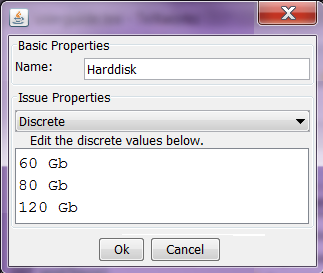
\includegraphics[width=0.95\textwidth]{media/image7a.png}
\caption{Creating a discrete issue.}
\label{fig:createIssueD}
\end{minipage}
\begin{minipage}[b]{0.55\linewidth}
	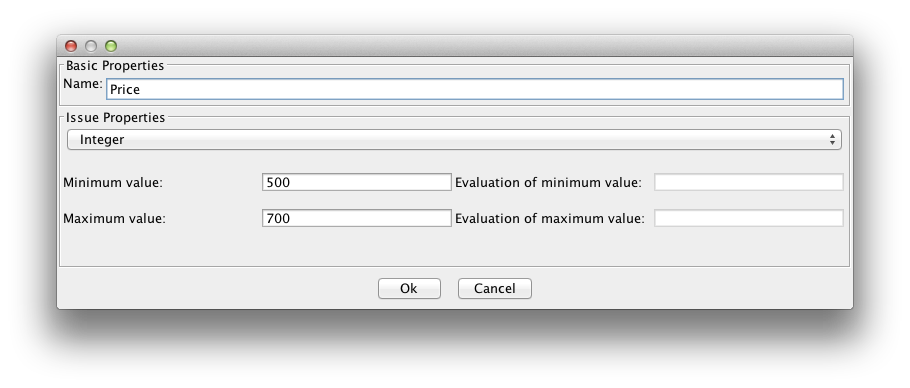
\includegraphics[width=1.0\textwidth]{media/image7b.png}
\caption{Creating an integer issue.}\label{fig:createIssueI}
\end{minipage}
\end{figure}

\subsection{Creating a Preference Profile}
Now that we created a domain, the next step is to add a set of preference profiles. By right clicking on the domain a popup menu is opened which has an option to create a new preference profile. Selecting this option results in the opening of a new window which looks similar to Figure~\ref{fig:utilcreated}.

\begin{figure}[htb]
	\centering
	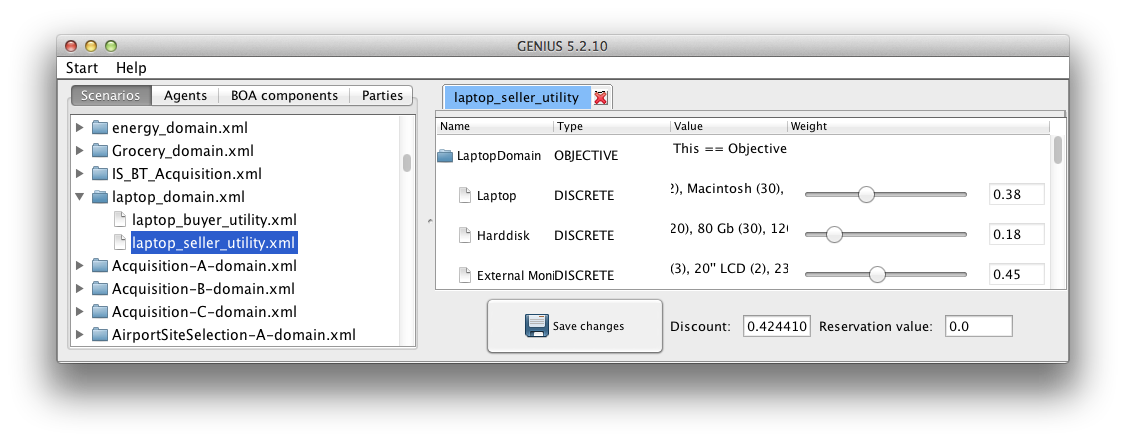
\includegraphics[width=0.8\textwidth]{media/laptop.png}
\caption{The negosimulator after creating a new utility space.}\label{fig:utilcreated}
\end{figure}

Now you are ready to start customizing the preference profile. There are three steps: setting the importance of the issues, determining the preference of the values of the issues, and configuring the reservation value and discount. To start with the first step, you can adjust the relative weights of the issues by using the sliders next to that issue. Note that when you move a slider, the weights of the other sliders are automatically updated such that the all weights still sum up to one. If you do not want that the weight of another issue automatically changes, you can lock its weight by selecting the checkbox behind it. Now that we set the weights of the issues, it is a good idea to save the utility space.

The next and final step is to set the evaluation of the issues. To specify the evaluation of an issue you can double click it to open a new window looking similar to Figure~\ref{fig:createIssueD} or Figure~\ref{fig:createIssueI} depending on the type of the issue.

For a discrete issue we need to specify the evaluation value of each discrete value. A specific value can be assigned any positive non-zero integer as evaluation value. During the negotiation the utility of a value is determined by dividing the value by the highest value for that particular issue. To illustrate, if we give 60 Gb evaluation 5, 80 Gb evaluation 8, and 120 Gb evaluation 10; then the utilities of these values are respectively 0.5, 0.8, and 1.0.

Specifying the preference of a integer issue is even easier. In this case we simply need to specify the utility of the lowest possible value and the highest possible value. The utility of a value in this range is calculated during the negotiation by using linear interpolation of the utilities of both given utilities.

The final step is to set the reservation value and discount of a preference profile. If you are satisfied with the profile you can save it by pressing ``Save changes''. Finally, you can create additional preference profiles for the domain and run a negotiation.


%=========================================================================================
\section{Running Negotiations}
This section discusses how to run a negotiation. There are a number of modes to run a negotiation:

\begin{itemize}
	\item \textbf{Negotiation session}. A negotiation session concerns a single negotiation in which two agents compete. This mode is mainly intended for new users.
	\item \textbf{Tournament}. A tournament is a collection of sessions. Two sets of agents compete against each other on a set of domains. The results of the sessions are stored in the ``log'' directory. These results can be more easily viewed by importing them into Excel and using pivot tables (cf. Section~\ref{sec:analysisExcel}).
	\item \textbf{Distributed tournament}. A distributed tournament is a tournament which is stored in a database and can therefore be divided among multiple computers to speed up calculation.
	\item \textbf{Multi-Party Negotiation}. A single negotiation session in which a number of agents (not necessarily 2) compete. Notice that this is a generalization of the simple Negotiation session above.
	\item \textbf{Multi-Party Tournament}. A tournament of multiparty sessions. Again, this is a generalization of the tournament above.
	
\end{itemize}

Before going into detail on how each of these modes work, we first discuss the two types of agents that can be used: automated agents and non-automated agents. Automated agents are agents that can compete against other agents in a negotiation without relying on input by a user. In general, these agents are able to make a large amount of bids in a limited amount of time.

In contrast, non-automated agents are agents that are fully controlled by the user. These types of agents ask the user each round which action they should make. \Genius~by default includes the UIAgent -- which has a simple user interface -- and the more extensive Extended UIAgent.


\subsection{Running a Negotiation Session}
To run a negotiation session select ``Start'' and then ``Negotiation Session''. This opens a window similar to Figure~\ref{Fig:session}. The following parameters need to be specified to run a negotiation:
\begin{itemize}
	\item \textbf{Negotiation protocol}. The set of available protocols. Normally ``Alternating Offers'' is used.
	\item \textbf{Side A/Side B}. The configuration of the agents of both sides.
	\item \textbf{Preference profile}. The preference profile to be used by the agent of that side.
	\item \textbf{Agent name}. The agent participating in the negotiation.
	\item \textbf{Deadline (seconds)}. The length of the negotiation in seconds.
\end{itemize}

\begin{figure}[h!]
	\centering
	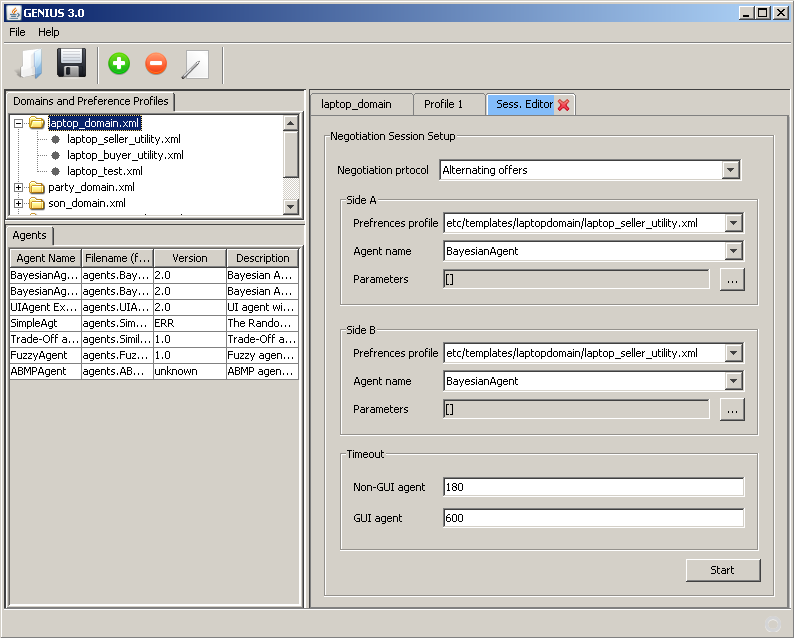
\includegraphics[width=0.65\textwidth]{media/image11.png}
\caption{A negotiation session.}\label{Fig:session}
\end{figure}


\subsection{Running a Tournament}\label{sec:runningTournament}
Besides running a single negotiation session, it is also possible to run a tournament. A tournament can be seen as a collection of sessions. In contrast to running a single session, the results of a tournament are stored in the ``log'' directory. These results can be easily analyzed by importing them into Excel (cf. Section~\ref{sec:analysisExcel}). A tournament can be created by first selecting ``Start'' and then ``Tournament''. The Tournament tab will appear similar to Figure~\ref{Fig:tournament}. This window shows a set of options which we need to specify. The value of an option can be specified by double clicking the option in the ``Values'' column.


\begin{figure}[htb]
	\centering
	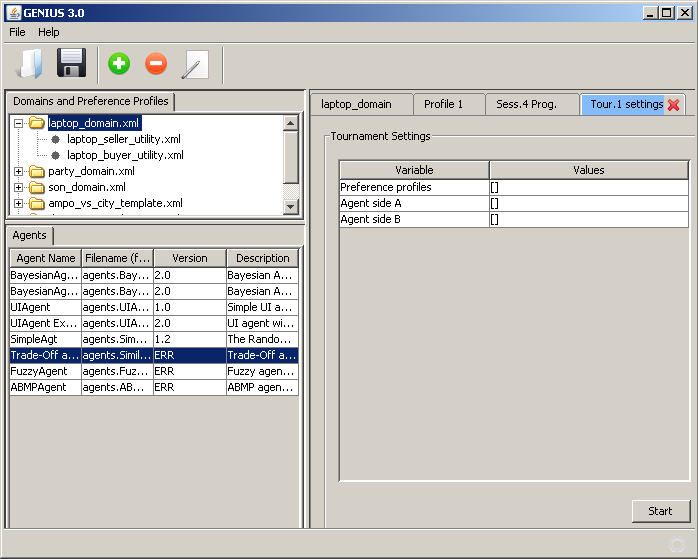
\includegraphics[width=0.9\textwidth]{media/image16.png}
\caption{Tournament tab.}\label{Fig:tournament}
\end{figure}

\begin{itemize}
	\item \textbf{Protocol}. The set of available protocols.
	\item \textbf{Preference profiles}. The set of scenarios on which the agents should compete. Each selected scenario should feature at least two preference profiles.
	\item \textbf{Agent side A/B}. The set of agents in set A competes against all agents in set B.
	\item \textbf{Number of sessions}. The number of times each session should be repeated.
	\item \textbf{Tournament options}. Options which specify how to run the tournament (see below).
	\item \textbf{BOA Agent side A/B}. Type of agents that consist of multiple components (see~Section~\ref{sec:boa}).
\end{itemize}

\subsubsection{Tournament Options}
A large set of tournament options can be specified which influence the composition and running of the tournament. There are four categories of options:

\begin{itemize}
	\item \textsc{Protocol settings} (Figure~\ref{fig:TourOptions1})
	\begin{itemize}
		\item \textbf{Protocol mode} . Specifies if the negotiation features rounds or time. In a time-based negotiation there is an amount of time to reach an agreement. Time passes while an agent deliberates an action. In contrast, in a rounds-based negotiation the deadline is specified in rounds. An agent can take more time to compute an action as time does not pass within a round.
		\item \textbf{Deadline}. Depending on the protocol mode, this is the maximum amount of time in seconds or amount of rounds. Note that one single round corresponds to one turn of a single agent.
		\item \textbf{Access partner preferences}. Allows agents to access the preference profile of the negotiation session, which contains the opponent's preference profile.
		\item \textbf{One-sided bidding} If enabled then agent A's bids are ignored, and replaced by the bid that has max utility for A. agent A's accepts are passed through.
		\item \textbf{Allow pausing timeline}. Allow agents to pause the negotiation by using the timeline.pause() and time.resume() methods.
	\end{itemize}
	\item \textsc{Session generation}(Figure~\ref{fig:TourOptions2})
	\begin{itemize}
		\item \textbf{Play both sides}. When generating the sessions, whether each pair of agents should play both sides on a scenario or not.
		\item \textbf{Play against self}. An agent may be included both in the set Agent side A and side B. If this option is enabled an agent is allowed to play against itself. If disabled, the sessions in which agents negotiate against themselves are removed.
		\item \textbf{Starting agent}. This agent has to place the first bid.
		\item \textbf{Generation mode}. Standard or Random. If set to random, the generated sessions are shuffled into a random order, using the random seed
		\item \textbf{Random seed}. Random seed used for shuffling sessions.
	\end{itemize}



		\begin{figure}[ht]
		\center
		\begin{minipage}[b]{0.4\linewidth}
			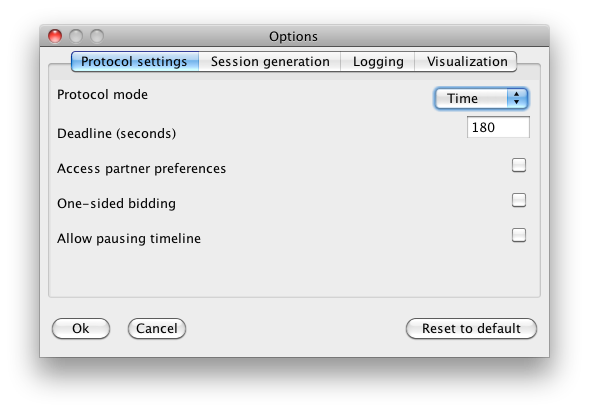
\includegraphics[width=0.95\textwidth]{media/TourOptions1.png}
		\caption{Protocol Settings.}
		\label{fig:TourOptions1}
		\end{minipage}
		\begin{minipage}[b]{0.4\linewidth}
			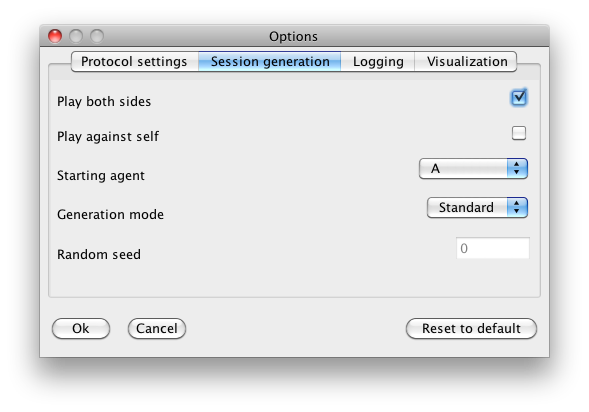
\includegraphics[width=0.95\textwidth]{media/TourOptions2.png}
		\caption{Session Generation options.}\label{fig:TourOptions2}
		\end{minipage}
		\end{figure}


	\item \textsc{Logging}(Figure~\ref{fig:TourOptions3})
	\begin{itemize}
		\item \textbf{Log detailed analysis}. Enabling this option activates a set of quality measures to capture the quality of the negotiation process. The quality measures are added to the default log. In addition, for the whole tournament an overview log is created. This log is prefixed with ``TM-''.
		\item \textbf{Log negotiation trace}. If enabled, a more extensive log is written including the bid history, to a file having the name {\tt "extensive\_log.xml"}. 
		\item \textbf{Log final accuracy} Logs the accuracy of the final opponent model of BOA agents on side A. This is done by comparing the opponent model of side A with the actual utility space of side B. Calculated are:
		\begin{itemize}
		\item the Pearson correlation coefficient by comparing the utility of each bid estimated by the real and estimated opponent's utility space. Higher is better.
		\item the ranking distance by comparing the utility of each bid estimated by the real and estimated opponent's utility space. Lower is better.
		\item the ranking distance by comparing the utility of each weight estimated by the real and estimated opponent's utility space. Lower is better.
		\item average difference between the real and estimated utility.
		\item average difference between the real and estimated issue weights.
		\item the absolute difference between the estimated Kalai point and the real Kalai point. Note that we are only interested in the value for the opponent.
		\item the absolute difference between the estimated Nash point and the real Nash point. Note that we are only interested in the value for the opponent.
		\item the average difference between the real estimated pareto bids and their estimated utility for the opponent.
		\item the amount of real Pareto bids which have been found by the opponent model. Note that the estimated utility space may have more or less Pareto bids than there really are.
		\item the percentage of bids in the estimated Pareto bids which is really Pareto optimal.
		\item  the Pareto frontier distance using the following steps: 1. Map the estimated Pareto-bids to the real space. 2. Calculate the surface beneath the real Pareto bids and estimated Pareto bids. 3. Subtract the surfaces and return the absolute difference. Note that the Pareto frontier difference can be positive and negative. In general, the mapped estimate of the Pareto frontier will have less surface; however, it can happen that less Pareto-points were estimated. In this case a Pareto-point is missed, and it can happen that the surface is therefore larger.

		\end{itemize}
		\item \textbf{Log competitiveness} this computes the amount of discrepancy between the two utility spaces. If X is the bid with maximum utility for side B, then {\em full yield of A} is the utility of X for side A.  The competitiveness ratio is defined as $CR(util)=1 - \frac{max(fullyield, util) - fullyield}{1 - fullyield}$. If this option is enabled, the following info is logged  for side A and side B
		\begin{itemize}
		\item full yield utility.
		\item BSCR = CR(minUtil) where minUtil is the minimum utility that an agent asked for (in one of its bids). 
		\item total CR. which equals to CR(final utility for this agent)
		\item ACCR =  total CR - BSCR.
		\item normalized ACCR = ACCR / (1 - BSCR)
		\end{itemize}
		\item \textbf{Append mode and deadline} appends the protocol mode and deadline (time or rounds) to the filename
	\end{itemize}
	\item \textsc{Visualization}(Figure~\ref{fig:TourOptions4})
	\begin{itemize}
		\item \textbf{Show all bids}. When enabled all bids in a scenario are visualized as red points in the negotiation status window. This option has some impact on performance.
		\item \textbf{Show last bid}. When enabled the last bid is marked with a special symbol to make it clear which move an agent performed.
		\item \textbf{Disable GUI}. When enabled most GUI elements are disabled. This speeds-up the negotiation up to a factor of 200 times. The progress of the tournament is printed to the console.
	\end{itemize}
\end{itemize}



		\begin{figure}[ht]
		\center
		\begin{minipage}[b]{0.4\linewidth}
			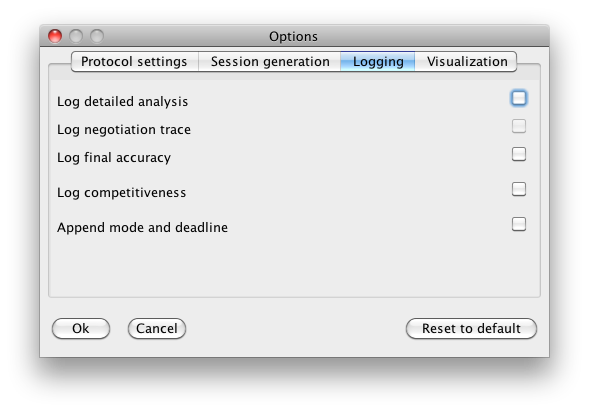
\includegraphics[width=0.95\textwidth]{media/TourOptions3.png}
		\caption{Protocol Settings.}
		\label{fig:TourOptions3}
		\end{minipage}
		\begin{minipage}[b]{0.4\linewidth}
			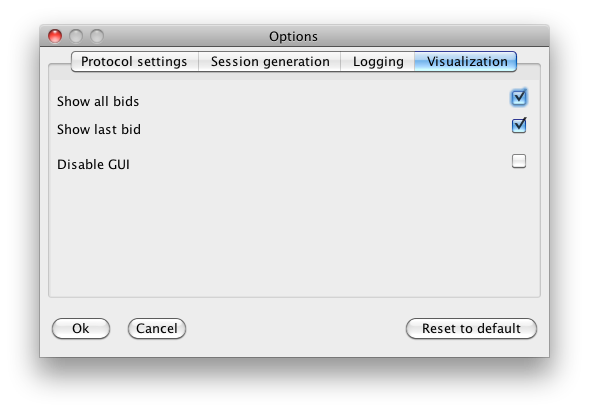
\includegraphics[width=0.95\textwidth]{media/TourOptions4.png}
		\caption{Session Generation options.}\label{fig:TourOptions4}
		\end{minipage}
		\end{figure}
		
		
\subsection{Advanced: Running a Distributed Tournament}
A tournament quickly becomes practically too large to run. Running a distributed tournament resolves this problem as the tournament is stored in a database. Next, instances of \Genius~-- perhaps running on the same computer -- can connect to the database and process part of the tournament.

Before we can run a distributed tournament, we first need to setup a simple MySQL server which can be accessed by the computers. The installation of the database should include the ``InnoDB'' database engine. We will use this engine because it allows us to more easily remove old tournament data that we no longer need. Furthermore we recommend at least 50 Mb of free space. The required database structure can be created by using the SQL dump which can be found in the directory \textit{doc/database}.

The next step is to specify a tournament to run. Towards this end, select ``Start'' and then ``Distributed tournament''. This opens a GUI similar to Figure~\ref{Fig:tournament}, except for the following four options:

\begin{itemize}
	\item \textbf{Database address}. The address of the database, for example \url{sql.ewi.tudelft.nl:3306/DG}.
	\item \textbf{Database user}. The username of the account for the database.
	\item \textbf{Database password}. The password of the user account for the database.
	\item \textbf{Database sessionname}. The identifier of the tournament. The identifier is needed as multiple distributed tournaments can be run at the same time.
\end{itemize}

After specifying the tournament and database parameters we can start the distributed tournament by pressing ``Start distributed tournament''. Selecting this button splits the tournament into smaller jobs which are stored in the database. The tournament is automatically started similar to a normal tournament. Now other computers can easily connect by specifying the database parameters and selecting ``Join distributed tournament''. For these computers we only need to fill in the database parameters as the configuration is loaded from the database. Finally, after running the full tournament the results are sent to all computers and stored in the ``log'' directory. Figure~\ref{fig:dtournament} summarizes the process.

\begin{figure}[htb]
	\centering
	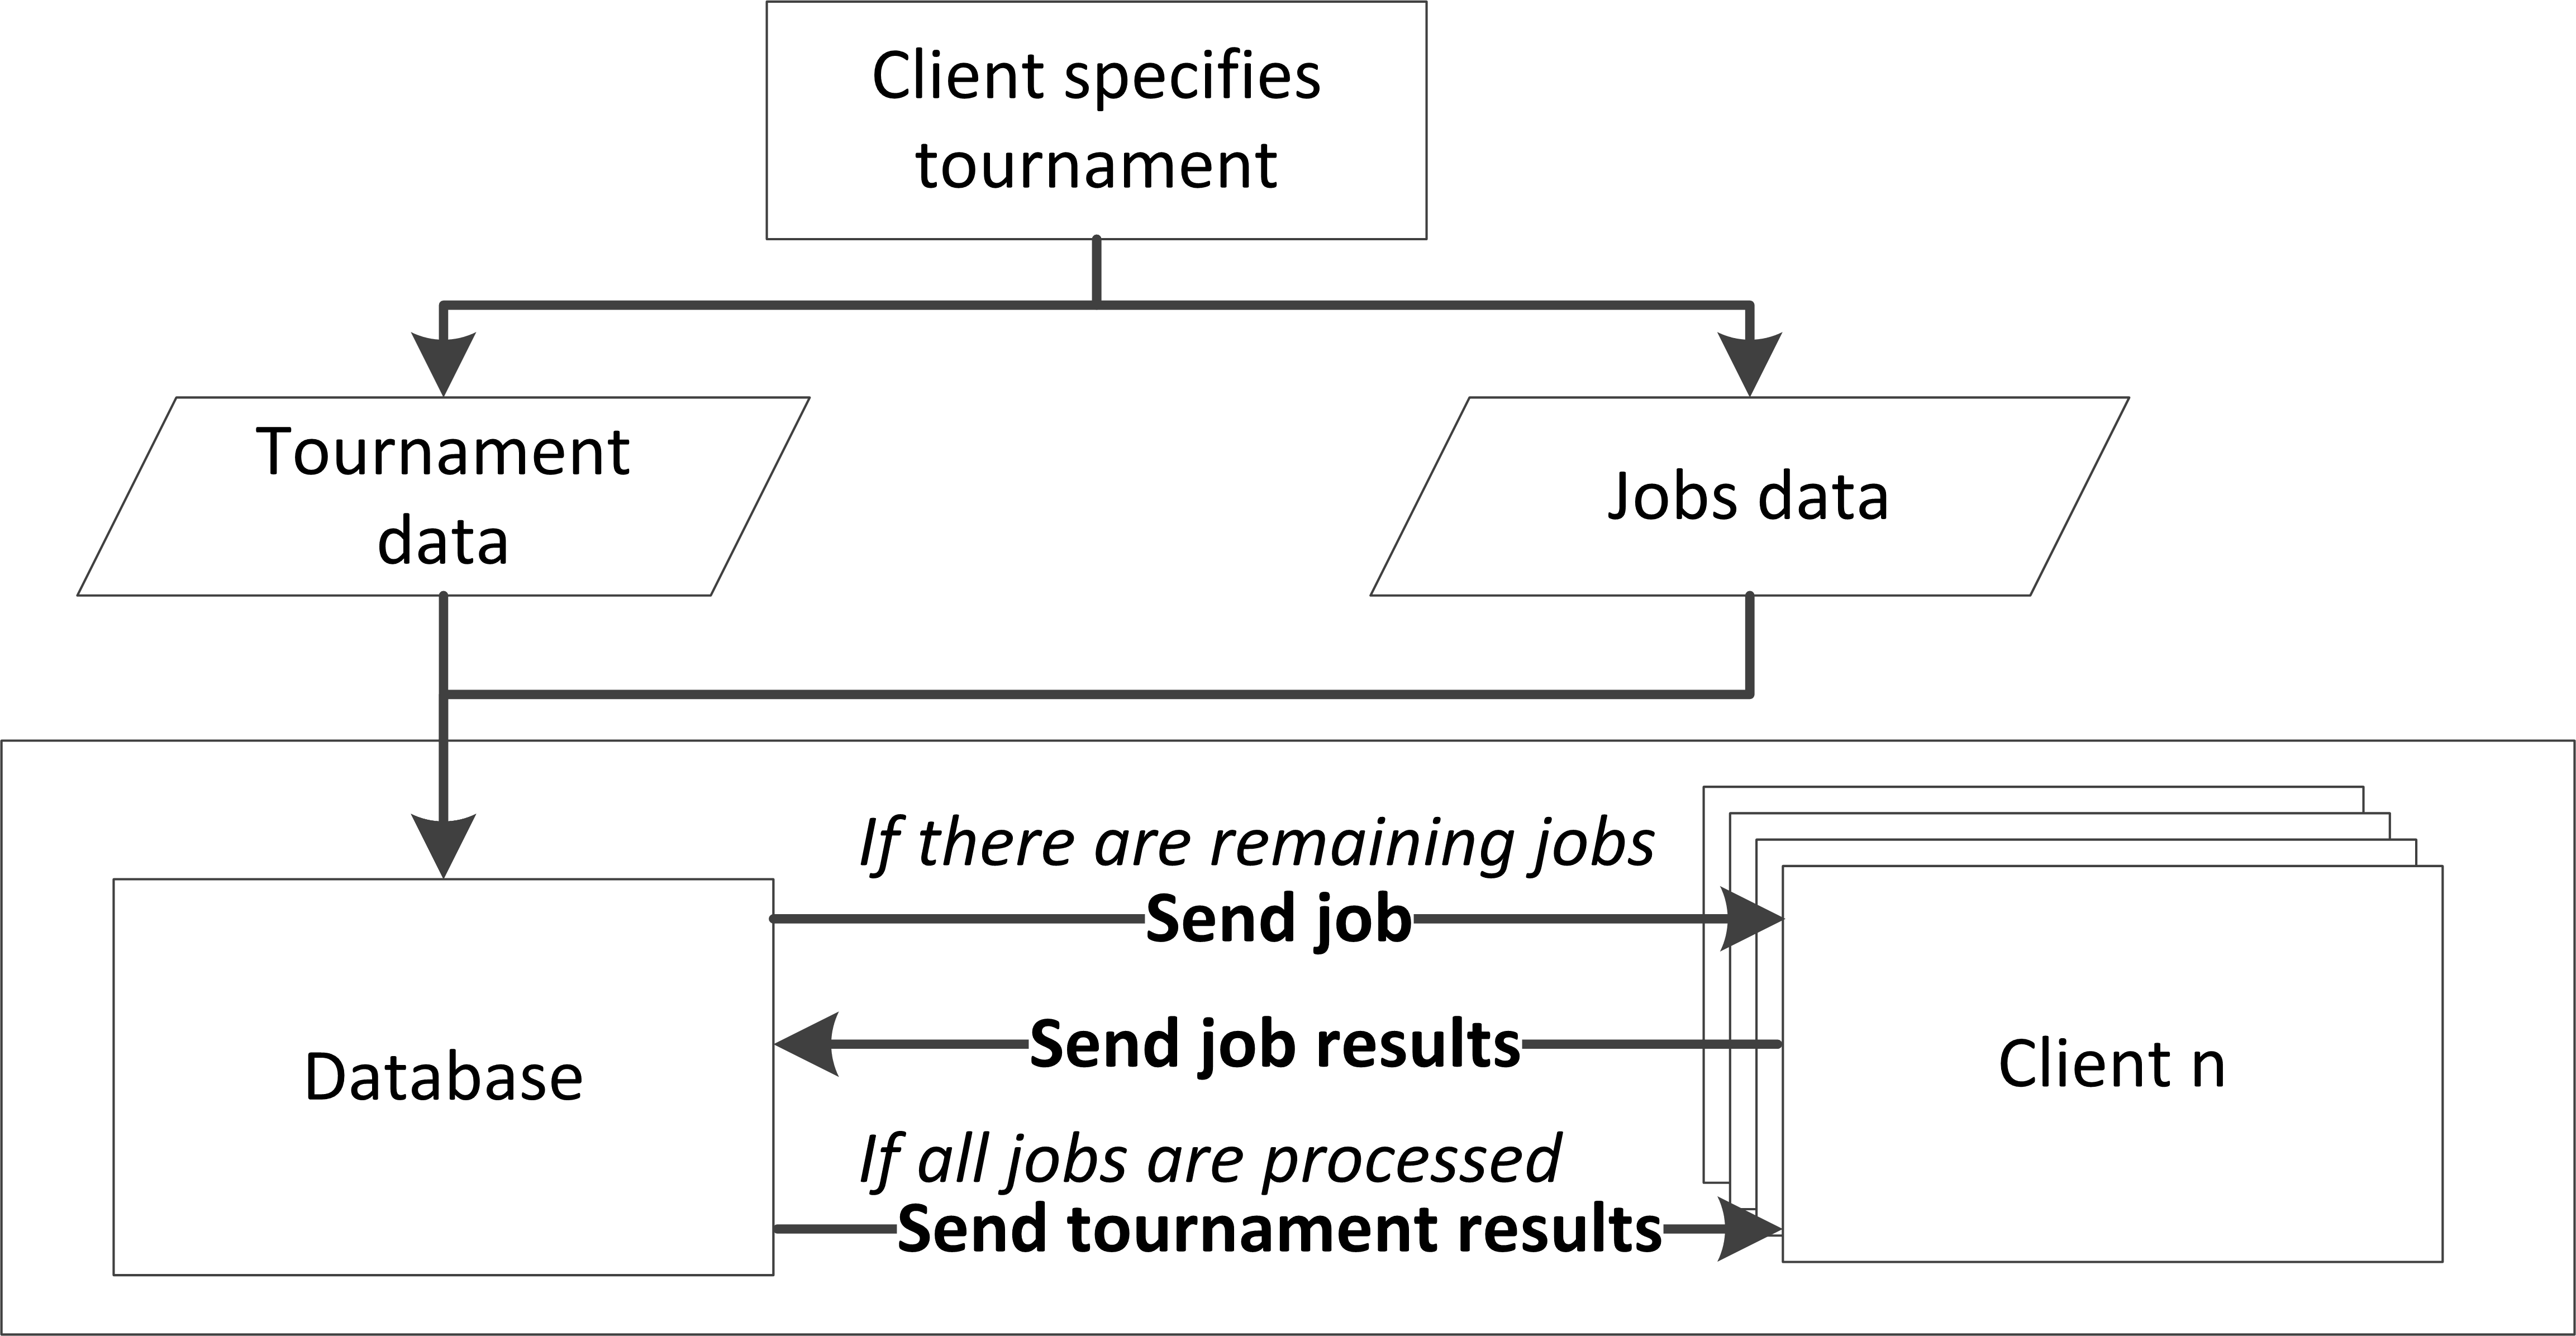
\includegraphics[width=0.50\textwidth]{media/DistributedGenius.png}
\caption{Distributed tournament process.}\label{fig:dtournament}
\end{figure}

It should be noted that currently there is no option in \Genius~to delete old tournament data. Therefore we recommend to install \textit{phpMyAdmin}. Using phpMyAdmin the old data of a tournament can be easily deleted by removing the tournament in the jobs table.



\subsection{Running a Multi-Party Negotiation}
To run a negotiation session select ``Start'' and then ``Multi-Party Negotiation''. This opens a window similar to Figure~\ref{Fig:multipartysession}. 


\begin{figure}[h!]
	\centering
	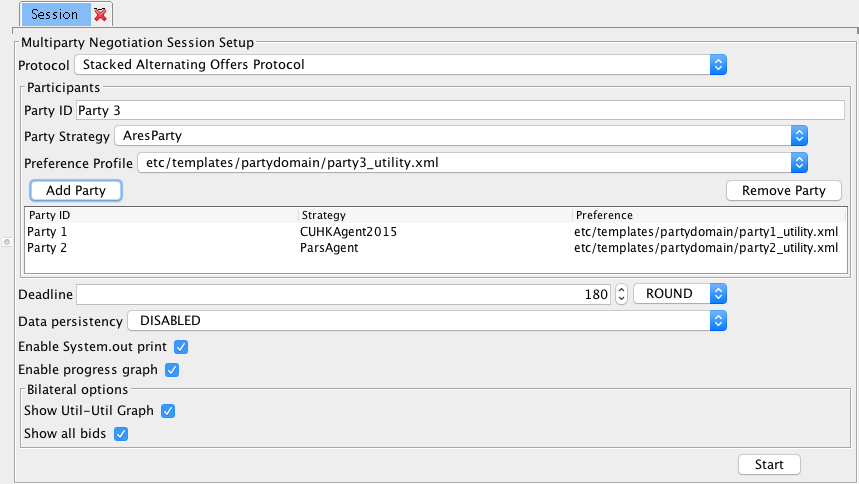
\includegraphics[width=0.5\textwidth]{media/multipartysession.png}
\caption{A multi-party negotiation session.}\label{Fig:multipartysession}
\end{figure}


The following parameters need to be specified to run a negotiation:

\medskip
\begin{minipage}{.8 \textwidth}
\begin{itemize}
	\item \textbf{Negotiation protocol}. The set of available protocols. Normally ``Alternating Offers'' is used.
	\item \textbf{A table with participants}. This table shows all currently added participants. 
	\item \textbf{Deadline Type}. The deadline in use. Can be "Round" or "Time".
	\item \textbf{Max duration}. The maximum duration of the session. The units are Round or Time as selected above.
\end{itemize}
\end{minipage}
\medskip

To modify the table of participants, you can either remove or add a party. 
To remove a party, select the party in the list and click the "Remove Party" button. To add a party, select the correct values for the next party:

\medskip
\begin{minipage}{.8 \textwidth}
\begin{itemize}
	\item \textbf{Party ID}. The name of the next party to be added.
	\item \textbf{Strategy}. The ID of the NegotiationParty (java class) to use for this party.
	\item \textbf{Preference profile}. The preference profile to be used by the next party to be added.
\end{itemize}
\end{minipage}
\medskip

After the correct settings have been set, press the "Add Party" button.

The negotiation is started when you press the start button. The tab contents will change to  a progress overview panel
showing you the results of the negotiation. The results are also stored in a log file.
 These results can be easily analyzed by importing them into Excel (cf. Section~\ref{sec:analysisExcel})


\subsection{Running a Multi-Party Tournament}
A multi-party tournament is a set of multi-party sessions. To prepare a multi-party tournament, select  ``Start'' and then ``Multi-Party Tournament''. 

\begin{figure}[htb]
	\centering
	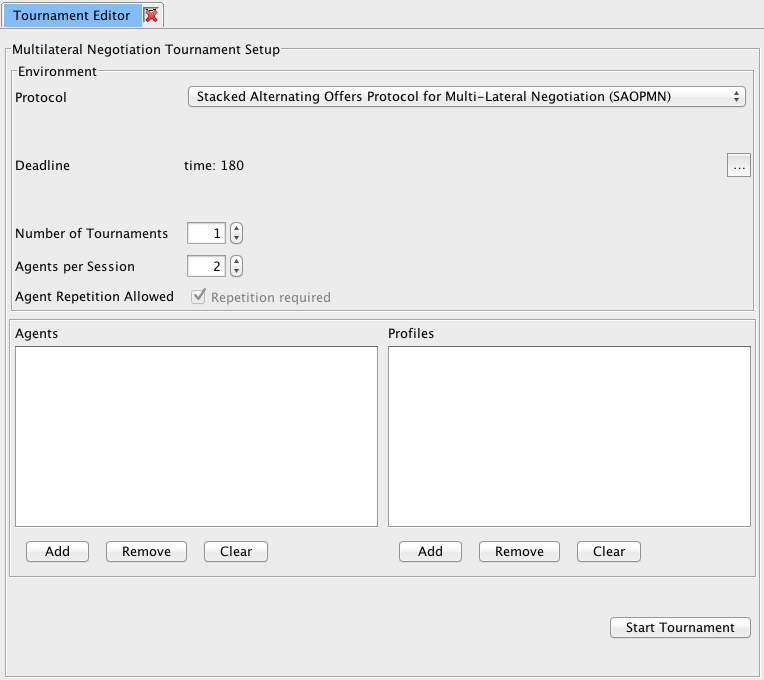
\includegraphics[width=0.5\textwidth]{media/multipartytournament.png}
\caption{Multi-Party Tournament}\label{Fig:multipartytournament}
\end{figure}

The Tournament tab will appear similar to Figure~\ref{Fig:multipartytournament}. This window shows a set of options which we need to specify:

\begin{itemize}
	\item \textbf{Protocol}. The protocol to use for each session.
	\item \textbf{Deadline}. The limits on time and number of rounds for each session.
	\item \textbf{Number of tournaments}. The number of times the entire tournament will be run.
	\item \textbf{Agents per Session}. The number of agents N to use for each session.
	\item \textbf{Agent Repetition Allowed}. Determines if agents are put back into the pool of agents after a run.
	\item \textbf{Agents}. The pool of agents to draw from. Click "Add" to select the set of agents to put into the pool. Select an agent and click "remove" to remove an agent from the pool. Click "Clear" to clear the pool.
	\item \textbf{Profiles}. The set of profiles to draw from. Click "Add" to select the set of profiles to put in the pool. Select a profile and click "Remove" to remove a profile from the pool. Click "Clear" to clear the pool. This option disables if there are more agents per session than the number of agents in the pool.
\end{itemize}

After you click "Start", the tournament starts. 

The parties (Agents) and profiles for each session are determined by created by all possible permutations of N agents from the agents pool (N is the number of Agents per Session) and permutations of N profiles from the profile pool. 
		
The results of the tournament are shown on screen and also stored in a log file.  These results can be easily analyzed by importing them into Excel (cf. Section~\ref{sec:analysisExcel})
	

\subsection{Running from the command line}
You can run a multi-party tournament from the command line, as follows.

\begin{enumerate}
\item Prepare an xml file that describes the settings for the tournament
\item Run the command runner and give it the prepared file 
\end{enumerate}

\subsubsection{Prepare the XML settings file}
Make a copy of the \verb|multilateraltournament.xml| file inside your genius directory and edit it (with a plain text editor).  Inside the \verb|<tournaments>| element you will find a number of \verb|<tournament>| elements. Each of these \verb|<tournament>| elements defines a complete tournament so you can run multiple tournaments using one xml file.

The contents of each \verb|<tournament>| element is as follows 

\begin{itemize}
    \item \textbf{deadline}. The deadline element contains two values:
      \begin{itemize}
        \item \textbf{value}. This is the maximum value determining the deadline. Must be an integer $\ge 1$.
        \item \textbf{type.} Can be either $ROUND$ or $TIME$. If $ROUND$, the value is the number of rounds. If $TIME$, value is a time in seconds.
      \end{itemize}
      
    \item \textbf{numSessions}. The number of times each session will be run in the tournament. 

    \item \textbf{numberOfAgentsPerSession}. The number of agents to be used for each session.
      
    \item \textbf{protocolItem}. Contains the information about the protocol. We recommend not to change this as there are no alternative protocols available at this moment.

    \item  \textbf{repetitionAllowed}. If true, agents from the partyRepItems negotiate against themselves in the sessions. 

    \item \textbf{partyRepItems}. This element contains a number of \verb|<item>| elements. Each of these party items contains the following:
      \begin{itemize}
        \item \textbf{protocolClassPath}. We do not support other protocols than negotiator.protocol.StackedAlternatingOffersProtocol at this moment.
        \item \textbf{description}A plain text description of this party
        \item \textbf{classPath} the java.party.class.path to the main class. That class must implement the NegotiationParty interface
        \item \textbf{partyName} the plain text name of the party
      \end{itemize}

    \item \textbf{partyProfileItems}. This element contains a number of items. There must be at least as much as numberOfAgentsPerSession. Each item element contains just the url that contains the description of that party profile. Usually these URIs have to point to files and therefore are of the form \verb|file:path/to/file.xml|
\end{itemize}

The tournament will consist of sessions created creating all permutations of \verb|<numberOfAgentsPerSession>| from the partyRepItems (with or without reuse, depending on \textbf{repetitionAllowed}. The randomization also is applied to the profile items.


\subsubsection{Run the tournament}
To run the tournament, open a terminal/console and change the working directory to the genius directory.
Then enter this command (where yourfile.xml is the name of the file you just edited):

\vspace{0.5cm}
\verb|java -cp negosimulator.jar negotiator.xml.multipartyrunner.Runner yourfile.xml|
\vspace{0.5cm}

Press return when the app prompts you for the log file location to log to  the default \verb|logs/...csv| file.

%=========================================================================================
\section{Quality Measures in Genius}\label{sec:qm}
A large set of quality measures have been incorporated in \Genius~ since version 4.0. Most quality measures are automatically available, while for others an option must be selected in the tournament options menu.

There are now two types of logs used in \Genius: the standard log and the tournament log. The standard log captures the outcome of each negotiation in a tournament by logging the results of the quality measures for both agents. The tournament log uses the standard log to calculate averages and standard deviations of functions of the quality measures in the standard log, for example the average final utility for all sessions which resulted in an agreement.

First, Section~\ref{sec:standardLog} discusses the measures incorporated in the standard log. Next, Section~\ref{sec:tournamentLog} details the tournament log. Finally, Section~\ref{sec:analysisExcel} discusses how Excel can be used to analyze logs.

\subsection{Overview of Quality Measures in the Standard Log}\label{sec:standardLog}
Since version 4.0, \Genius~ incorporates two types of quality measures: standard measures and detailed measures. In addition there are some experimental measure types, such as competitiveness and opponent model accuracy, however these are not discussed here. In the following sections we discuss both measure types in detail.

\subsubsection{Standard Measures}
The standard measures are the measures which are enabled by default and cannot be disabled. Table~\ref{tab:standardmeasures} provides an overview of all default quality measures.

\begin{table}[h!]
	\small
	\center
	\begin{tabular}{|p{4.7cm}|p{9.2cm}|}
		\hline\hline
		\textbf{Attribute} & \textbf{Description}\\[-0.2ex] 
		\hline\hline
		acceptance\_strategy & The acceptance strategy of a BOA agent~(see Section~\ref{sec:boa}). \\[-0.2ex]\hline
		agent & The side at which the agent played (A or B). \\[-0.2ex]\hline
		agentClass & The classpath of the agent. \\[-0.2ex]\hline
		agentName & The name of the agent. \\[-0.2ex]\hline
		bestAcceptableBid & Utility of the best bid offered to the agent. Note that the discount is not taken into account. \\[-0.2ex]\hline
		bestDiscountedAccepableBid & Utility of the best bid offered to the agent, taking the discount into account. \\[-0.2ex]\hline
		bids & Amount of offers exchanged during the negotiation. \\[-0.2ex]\hline
		currentTime & Time of storage of the result of the negotiation. \\[-0.2ex]\hline
		discountedUtility & The discounted utility earned by the agent in the negotiation. \\[-0.3ex]\hline
		domain & Domain at which the negotiation took place.\\[-0.3ex]\hline
		errors & Errors encountered during the negotiation. Not reaching an agreement before the deadline is also treated as an error.\\[-0.3ex]\hline
		finalUtility & The undiscounted utility earned by the agent in the negotiation.\\[-0.3ex]\hline
		lastAction & Last action made before the negotiation ended.\\[-0.3ex]\hline
		normalized\_utility & The final utility divided by the maximum possible utility according to the preference profile. In correct domains the result should be equal to the final utility.\\[-0.3ex]\hline
		offering\_strategy & The offering strategy of a BOA agent~(see Section~\ref{sec:boa}). \\[-0.3ex]\hline
		opponent-agentClass & The classpath of the opponent.\\[-0.3ex]\hline
		opponent-agentName & The name of opponent's agent.\\[-0.3ex]\hline
		opponent\_model & The opponent model of a BOA agent~(see Section~\ref{sec:boa}). \\[-0.3ex]\hline
		opponent-utilSpace & The opponent's preference profile.\\[-0.3ex]\hline
		runNumber & How many times the negotiation has been repeated before.\\[-0.3ex]\hline
		startingAgent & Side which started the negotiation: A or B.\\[-0.3ex]\hline
		timeOfAgreement & Normalized time at which an agreement was established. 1.0 for no agreement. \\[-0.3ex]\hline
		utilSpace & The agent's preference profile.\\[-0.3ex]
		\hline
		\hline
	\end{tabular}
	\caption{Standard quality measures in \Genius~in alphabetic order.}
	\label{tab:standardmeasures}
\end{table}

\subsubsection{Detailed Measures}\label{sec:detailedmeasures}
The detailed quality measures consist of trajectory analysis measures and measures for the fairness and optimality of the outcome. The detailed measures can be enabled by selecting ``Log detailed analysis'' in the tournament options menu. Enabling this option also results in the generation of the tournament log discussed in Section~\ref{sec:tournamentLog}.

\begin{table}[h!]
	\small
	\center
	\begin{tabular}{|p{4.7cm}|p{9.2cm}|}
		\hline\hline
		\textbf{Attribute} & \textbf{Description}\\[-0.2ex] 
		\hline\hline
		concession\_moves & The percentage of moves in which the agent, relative to the previous offer, offered a bid with decreased its own utility and increased its opponent's utility.\\[-0.3ex]\hline
		exploration\_rate & The percentage of bids in the outcome space explored by the agent. Two bids with exactly the same utilities for both parties are treated as a single same bid.\\[-0.3ex]\hline
		fortunate\_moves & The percentage of moves in which the agent, relative to the previous offer, offered a bid which increased both its own and its opponent's utility.\\[-0.3ex]\hline
		joint\_exploration\_bids & The percentage of unique bids of the outcome space explored by both agents together. Two bids with exactly the same utilities for both parties are treated as a single same bid. \\[-0.3ex]\hline
		kalai\_distance & Distance from the undiscounted utilities of the outcome to the Kalai-Smorodinsky solution.\\[-0.3ex]\hline
		nash\_distance & Distance from the undiscounted utilities of the outcome to the Nash solution. \\[-0.3ex]\hline
		nice\_moves & The percentage of moves in which the agent, relative to the previous offer, offered a bid which increased its opponent's utility without significantly changing its own utility.\\[-0.3ex]\hline
		pareto\_distance & Distance from the undiscounted utilities of the outcome to the nearest bid on the Pareto-optimal frontier.\\[-0.3ex]\hline
		perc\_pareto\_bids & Percentage of Pareto-optimal bids offered by an agent.\\[-0.3ex]\hline
		selfish\_moves & The percentage of moves in which the agent, relative to the previous offer, offered a bid which increased its own utility and decreased its opponent's utility.\\[-0.3ex]\hline
		silent\_moves & The percentage of moves in which the agent, relative to the previous offer, offered a bid which which was (nearly) equally valued by both agents.\\[-0.3ex]\hline
		social\_welfare & A fairness measure being the sum of the utilities for both agents.\\[-0.3ex]\hline
		unfortunate\_moves & The percentage of moves in which the agent, relative to the previous offer, offered a bid which decreased both its own and its opponent's utility.\\[-0.3ex]
		\hline
		\hline
	\end{tabular}
	\caption{Detailed quality measures in \Genius~in alphabetic order.}
	\label{tab:detailedMeasures}
\end{table}

\begin{comment}
\subsubsection{Opponent Model Accuracy Measures}
Log final accuracy

\begin{table}[h!]
\small
	\center
\begin{tabular}{|p{4.7cm}|p{9.2cm}|}
\hline
\textbf{Attribute} &\textbf{Description}\\
\hline\hline
\textsl{Pearson\_Correlation\_Bids} & Pearson correlation coefficient between real and estimated preference profile.\\
\hline
\textsl{Ranking\_Distance\_Bids} & Ranking distance between real and estimated preference profile.\\
\hline
\textsl{Average\_Difference\_Bids} & Average difference between the real and estimated utility of each possible bid.\\
\hline
\textsl{Ranking\_Distance\_Issue\_Weights} & Ranking distance between real and estimated issue weights.\\
\hline
\textsl{Average\_Difference\_Issue\_Weights} & Average difference between the real and estimated issue weights.\\
\hline
\textsl{Kalai\_Difference} & Difference between the real and estimated utility of the Kalai-point.\\
\hline
\textsl{Nash\_Diference} & Difference between the real and estimated utility of the Nash-point.\\
\hline
\textsl{Difference\_Pareto\_Frontier} & The average difference between the real and estimated utility for each Pareto bid.\\
\hline
\textsl{Percentage\_Correct\_Pareto\_Bids} & Percentage of real Pareto bids which are also estimated to be a Pareto bid.\\
\hline
\textsl{Percentage\_Incorrect\_Pareto\_Bids} & Percentage of estimated Pareto bids which are also real Pareto bids.\\
\hline
\textsl{Pareto\_Frontier\_Distance} & First, the position of the estimated Pareto bids is determined in the real space. The value of the measure is the absolute difference in surface under the real Pareto bids and the bids estimated to be Pareto optimal.\\ % absolute, because if a point is missed, then surface of estimate can actually be larger. Note that this case is rare
\hline
\end{tabular}
	\caption{Opponent model accuracy measures in \Genius~in alphabetic order.}
	\label{tab:omaccuracyMeasures}
\end{table} 
\end{comment}

\subsection{Overview of Quality Measures in the Tournament Log}~\label{sec:tournamentLog}
The tournament log is an analysis of the results on the quality measures for each agent, for example the average utility for \textit{Agent K}. Similar to the detailed quality measured the tournament log can be enabled by selecting ``Log detailed analysis'' in the tournament options menu.

Three types of measures are included in the log:
\begin{itemize}
	\item \textbf{Averages of quality measures}. The tournament log includes a large set of averages of the quality measures in the standard log. Examples include the average Nash distance, the average percentage of silent moves, and the average social welfare.
	\item \textbf{Standard deviations of quality measures}. The tournament log also includes the standard deviation of some measures. Note that this not the normal standard deviation of for example the utility, but the more complicated deviation between runs. To illustrate, if there were ten runs of the tournament, then each run has an average utility and we can calculate the standard deviation of this utility between runs.
	\item \textbf{Average of functions of quality measures}. The tournament log also includes a large set of measures which are functions of measures included in the standard log. An example is the average utility for an agent only for the matches which resulted in agreement. 
\end{itemize}

\subsection{Analyzing Logs using Excel}~\label{sec:analysisExcel}
The logs are in XML format, which entails that we can easily analyze them by using Excel. Note that the following discussion does not apply to the starter edition of Excel, as it does not support Pivot tables.

The XML data of the standard log can be converted to a normal table by importing the data into Excel using the default options. This results in a large table showing the result for both agents A and B for each session. Analyzing these results manually is complicated, therefore we recommend to use pivot tables. Pivot tables allow to summarize a large set of data using statistics and can be created by selecting ``Insert'' and then ``Pivot Table''. To illustrate, by dragging the \textit{agentName} in ``Row Labels'' and the \textit{discountedUtility} in ``Values'' (see Figure~\ref{fig:pivottable}), we can easily see which agent scored best in the tournament. If solely the amount of matches of each agent is displayed, you need to set the ``Value Field Settings'' of \textit{discountedUtility} to average instead of count.

\begin{figure}[htb]
	\centering
	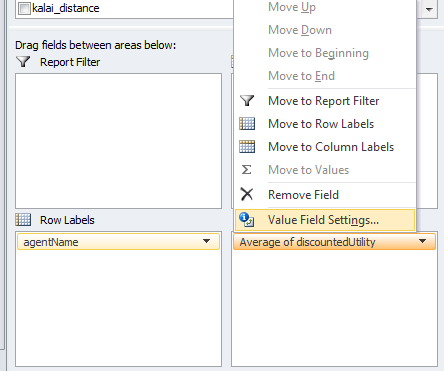
\includegraphics[width=0.4\textwidth]{media/PivotTable.png}
\caption{Configuration required to summarize the discounted utility of each agent.}\label{fig:pivottable}
\end{figure}



%=========================================================================================
\section{Setting up Java and IDE}
We assume that you are familiar with programming in Java. In case you are not familiar with Java, please consult the following tutorial: 

\texttt{http://www.oracle.com/technetwork/java/javase/documentation/index.html} 

The Java API definitions can be found here as well.

The recommended way to develop an agent is to create a new project in for example Eclipse or Netbeans. 
To develop \Genius components, you will need to add the \textit{negosimulator.jar} as an external library to the project such that classes in the project can use the classes of \Genius. You can copy the negosimulator.jar from the zip file into your project space.

In the examples we will use manual compilation to avoid the need to discuss IDE peculiarities.



%=========================================================================================
\section{Creating a Bilateral Negotiation Agent}
This section discusses how to create a basic bilateral negotiation agent in Java. Bilateral means you can only use this agent in a two-party negotation but not in a multi-party negotiation. A standard negotiation agent implements an agent as a single block of logic: a mix of a bidding strategy, acceptance strategy, and possibly an opponent model. In contrast, we recommend to separately implement these components to create a BOA agent as discussed in Section~\ref{sec:boa}. The main advantage of a BOA agent is that existing components can be reused, allowing for easier agent development.

Finally, to create an agent create a new class and extend the \textit{negotiator.Agent} class. Table~\ref{tab:agentclass} shows the most important fields and methods of this class. For more information, please refer to the javadoc of \Genius. To implement your agent, you have to override the three methods: \textit{receiveMessage}, \textit{init}, and \textit{chooseAction}. An agent may consist of multiple classes as long as one class extends the \textit{negotiator.Agent} class.

\begin{table}[h]
\begin{tabular}{m{0.9\textwidth}}
\hline
\texttt{UtilitySpace utilitySpace}\\
The preference profile of the scenario allocated to the agent.\\
\hline
\texttt{Timeline timeline}\\
Use timeline for every time-related by using \texttt{getTime()}.\\
\hline
\texttt{double getUtility(Bid bid)}\\
A convenience method to get the utility of a bid taking the discount factor into account.\\
\hline
\texttt{void init()}\\
Informs the agent about beginning of a new negotiation session.\\
\hline
\texttt{void ReceiveMessage(Action opponentAction)}\\
Informs the agent which action the opponent did.\\
\hline
\texttt{Action chooseAction()}\\
This function should return the action your agent wants to make next.\\
\hline
\texttt{String getName()}\\
Returns the name of the agent. Please override this to give a proper name to your agent.\\
\hline
\end{tabular}
\caption{The most important methods and fields of the Agent class.}
\label{tab:agentclass}
\end{table}

\subsection{Receiving the Opponent's Action}\label{sec:receiveAction}
The \texttt{ReceiveMessage(Action opponentAction)} informs you that the opponent just performed the action \texttt{opponentAction}. The \texttt{opponentAction} may be  \texttt{null} if you are the first to place a bid, or an \texttt{Offer}, \texttt{Accept} or \texttt{EndNegotiation} action.
The \texttt{chooseAction()} asks you to specify an \texttt{Action} to send to the opponent.

In the SimpleAgent code, the following code is available for \texttt{ReceiveMessage}. The SimpleAgent stores the opponent's action to use it when choosing an action.

\begin{lstlisting}
public void ReceiveMessage(Action opponentAction) {
	actionOfPartner = opponentAction;
}
\end{lstlisting}

\subsection{Choosing an Action}\label{sec:chooseAction}
The code block below shows the code of the method \texttt{chooseAction} for SimpleAgent. For safety, all code was wrapped in a try-catch block, because if our code would accidentally contain a bug we still want to return a good action (failure to do so is a protocol error and results in a utility of 0.0).

The sample code works as follows. If we are the first to place a bid, we place a random bid with sufficient utility (see the .java file for the details on that). Else, we determine the probability to accept the bid, depending on the utility of the offered bid and the remaining time. Finally, we randomly accept or pose a new random bid.

While this strategy works, in general it will lead to suboptimal results as it does not take the opponent into account. More advanced agents try to model the opponent's strategy or preference profile.

\begin{lstlisting}
public Action chooseAction() {
	Action action = null;
	try { 
		if (actionOfPartner == null) {
			action = chooseRandomBidAction();
		}
		if (actionOfPartner instanceof Offer) {
			Bid partnerBid = ((Offer) actionOfPartner).getBid();
			double offeredUtilFromOpponent = getUtility(partnerBid);
			// get current time
			double time = timeline.getTime();
			action = chooseRandomBidAction();
			
			Bid myBid = ((Offer) action).getBid();
			double myOfferedUtil = getUtility(myBid);
			
			// accept under certain circumstances
			if (isAcceptable(offeredUtilFromOpponent,myOfferedUtil,time)) {
				action = new Accept(getAgentID());
			}
		}
	} catch (Exception e) { 
		e.printStackTrace();
		action = new Accept(getAgentID()); // best guess if things go wrong. 
	}
	return action;
}
\end{lstlisting}

The method \textit{isAcceptable} implements the probabilistic acceptance function$P_\text{accept}$:

\begin{equation}
	P_\text{accept} = \dfrac{u - 2ut + 2\left(t - 1 + \sqrt{(t - 1)^2 + u(2t - 1)}\right)}{2t - 1}
\end{equation}
where $u$ is the utility of the bid made by the opponent (as measured in our utility space), and $t$ is the current time as a fraction of the total available time. Figure~\ref{Fig:Paccept} shows how this function behaves depending on the utility and remaining time. Note that this function only decides if a bid is acceptable or not. More advanced acceptance strategies also use the \texttt{EndNegotiation} action.
\begin{figure}[htb]
	\centering
	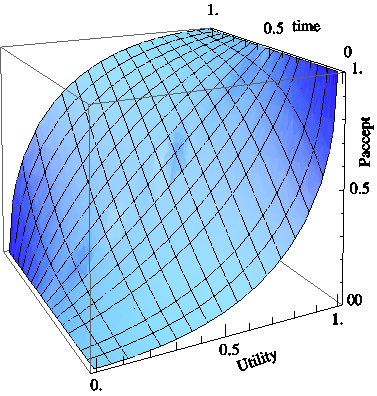
\includegraphics[width=0.3\textwidth]{media/image21.png}
	\caption{$P_\text{accept}$ value as function of the utility and time (as a fraction of the total available time).}\label{Fig:Paccept}
\end{figure}
%\subsection{Init}
%An important consideration for the implementation is that an agent may participate in multiple negotiation sessions with the same opponent. This enables the agent to learn from the previous sessions. For this reason, the negotiation environment calls the method \texttt{init} before starting the new session.
 
Automatic agents have to negotiate on their own, and are not allowed to communicate with a human user. Therefore, do not override the \texttt{isUIAgent()} function in automatic negotiation agents.

\subsection{General properties}
Some agents have restrictions and can not be used in certain situations. 
The agent indicates its capabilities through the function getSupportedNegotiationSetting().
By default, the agent has no restrictions. If your agent has restrictions, you must override
this function and return the appropriate supported settings.

For example, if your agent can only handle linear utility spaces, you should override like this

\begin{lstlisting}
	@Override
	public SupportedNegotiationSetting getSupportedNegotiationSetting() {
		return SupportedNegotiationSetting.getLinearUtilitySpaceInstance();
	}
\end{lstlisting}

\subsection{Overview of Classes}
This section provides an overview of classes which might be useful when implementing an agent. For the documentation of the data structures that are presented, please refer to the Javadoc that can be found in your download of \Genius. 

\begin{itemize}

\item \textbf{BidDetails} is a structure to store a bid and its utility.
\item \textbf{BidDetailsTime} is a structure to store a bid, its utility, and the time of offering.
\item \textbf{BidHistory} is a structure to keep track of the bids presented by the agent and the opponent.
\item \textbf{BidIterator} is a class used to enumerate all possible bids. Also refer to \textit{SortedOutcomeSpace}.
\item \textbf{BidSpace} is a class which can be used to determine the Pareto-optimal frontier and outcomes such as the Nash solution. This class can be used with the opponent's utility space as estimated by an opponent model.
\item \textbf{Pair} is a simple pair of two objects.
\item \textbf{Range} is a structure used to describe a continuous range.
\item \textbf{SortedOutcomeSpace} is a structure which stores all possible bids and their utilities by using BidIterator. In addition, it implements efficient search algorithms that can be used to search the space of possible bids for bids near a given utility or within a given utility range.
\item \textbf{UtilitySpace} is a representation of a preference profile. It is recommended to use this class when implementing a model of the opponent's preference profile.
\end{itemize}

\subsection{Compiling an Agent}
Compiling an agent can be done as follows (here we compile the examplepackage; modify as appropriate for your agent):
\begin{itemize}
\item Open a terminal
\item Switch to the root directory of genius
\item execute the command \texttt{javac -cp negosimulator.jar -source 1.6 -target 1.6  examplepackage/ExampleAgent.java}
\end{itemize}

You can also compile from Eclipse or Netbeans. Make sure you add the negosimulator.jar to your class path. Please refer to the Eclipse or Netbeans documentation on how to do this. Also you can check our tutorial on how to do this from Eclipse.

\subsection{Loading an Agent}
The next step is to load the compiled agent in \Genius. We can add the agent in one of the following two ways:

\begin{itemize}	
\item \textbf{Loading the agent using the GUI}. An agent can be easily added by going to the ``Agents'' tab in the ``Components Window'' (see Figure~\ref{fig:addAgent}). Next, pressing right click opens a popup with the option to add a new agent. The final step is to select the main class of your agent.

\begin{figure}[h] 
	\center
	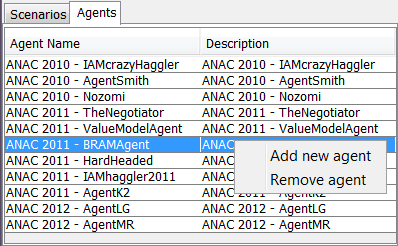
\includegraphics[width=5.5cm]{media/AddAgent.png}
	\caption{Adding an agent using the GUI.}
	\label{fig:addAgent}
\end{figure}

\item \textbf{Loading the agent using XML}. A compiled agent can also be loaded by directly adding the agent to the repository using the \textit{agentrepository.xml} file. The code below visualizes a repository with a single agent. An agent element consists of several subelements. the first element is the \textit{description} of the agent which is visualized in the GUI. The second element is the \textit{classPath} specifying were the compiled agent class is located. For built-in agents this is the class name but for user-defined agents this is the full filename of the main class of the agent (the one implementing the Agent interface). The third element specifies the \textit{agentName}. The optional element \textit{params} specifies the parameters and their values available to the agent. In this case, a parameter ``e'' with value 2 and a parameter ``time'' with value 0.95 is specified. Variables can be accessed during the negotiation by using the \textit{getStrategyParameters} method.
\end{itemize}

\begin{lstlisting}
<?xml version="1.0" encoding="UTF-8" standalone="yes"?>
<repository fileName="agentrepository.xml">
  <items>
   <agentRepItems>
               <agentRepItem description="Simple Agent" 
               classPath="/Users/wouter/Desktop/genius/examplepackage/ExampleAgent.class"
               agentName="Simple Agent"/>
               params="e=2;time=0.95"/>
     </agentRepItems>
  </items>
<filename>agentrepository.xml</filename>
</repository>
\end{lstlisting}




\subsection{Creating a ANAC2013 Agent}\label{sec:anac2013agent}
The ANAC2013 introduces the concept that an agent can save and load information for each preference profile. This entails that an agent can learn from previous negotiations, against the same opponent or multiple opponents, to improve its competence when having a specific preference profile. It is only possible to retrieve information learned on the current preference profile as to avoid having perfect knowledge about the opponent's preferences.

A single serializable object can be saved per preference profile by using the \textit{saveSessionData} method. If an object was already saved for the preference profile it is replaced. We recommend to store objects in the \textit{endSession} method, which is called when a negotiation is finished. The saved object can be requested by using the \textit{loadSessionData} method. A good place to do so is in in the \textit{init} method. Note that this functionality is also available to BOA agents (cf.\ Section~\ref{sec:anac2013agentBOA}).


%=========================================================================================
\section{Creating a BOA Agent}\label{sec:boa}
Instead of implementing your negotiating agent from scratch, we recommend you create a BOA agent using the \textit{BOA framework}. The BOA negotiation agent architecture allows to reuse existing components from other BOA agents. Many of the sophisticated agent strategies that currently exist are comprised of a fixed set of modules. Generally, a distinction can be made between four different modules: one module that decides whether the opponent's bid is acceptable (\textit{acceptance strategy}); one that decides which set of bids could be proposed next (\textit{bidding strategy}); one that tries to guess the opponent's preferences (\textit{opponent model}), and finally a component which specifies how the opponent model is used to select a bid for the opponent (\textit{opponent model strategy}). The overall negotiation strategy is a result of the interaction between these components.

The advantages of separating the negotiation strategy into these four components (or equivalently, fitting an agent into the BOA framework) are threefold: first, it allows to \textit{study the performance of individual components}; second, it allows to \textit{systematically explore the space of possible negotiation strategies}; third, the reuse of existing components \textit{simplifies the creation of new negotiation strategies}.

\subsection{Components of the BOA Framework}
A negotiation agent in the BOA framework, called a \textit{BOA agent}, consists of four components:
\begin{description}
  \item[Bidding strategy] A bidding strategy is a mapping which maps a negotiation trace to a bid. The bidding strategy can interact with the opponent model by consulting with it.%, passing one or multiple bids and see how they compare within the opponent's utility space.

  \item[Opponent model] An opponent model is in the BOA framework a learning technique that constructs a model of the opponent's preference profile.% In our approach, the opponent model should be able to estimate the opponent's utility of a given bid.
  \item[Opponent model strategy] An opponent model strategy specifies how the opponent model is used to select a bid for the opponent and if the opponent model may be updated in a specific turn.
  \item[Acceptance strategy] The acceptance strategy determines whether the opponent's bid is acceptable and may even decide to prematurely end the negotiation.
\end{description}
The components interact in the following way (the full process is visualized in Figure~\ref{fig:flowchart}). When receiving a bid, the BOA agent first  updates the \textit{bidding history}. Next, the \textit{opponent model strategy} is consulted if the \textit{opponent model} may be updated this turn. If so, the \textit{opponent model} is updated.

Given the opponent's bid, the \textit{bidding strategy} determines the counter offer by first generating a set of bids with a similar preference for the agent. The \textit{bidding strategy} uses the \textit{opponent model strategy} to select a bid from this set taking the opponent's utility into account.

Finally, the \textit{acceptance strategy} decides whether the opponent's action should be accepted. If the opponent's bid is not accepted by the acceptance strategy, then the generated bid is offered instead.

\begin{figure}[t] 
	\center
	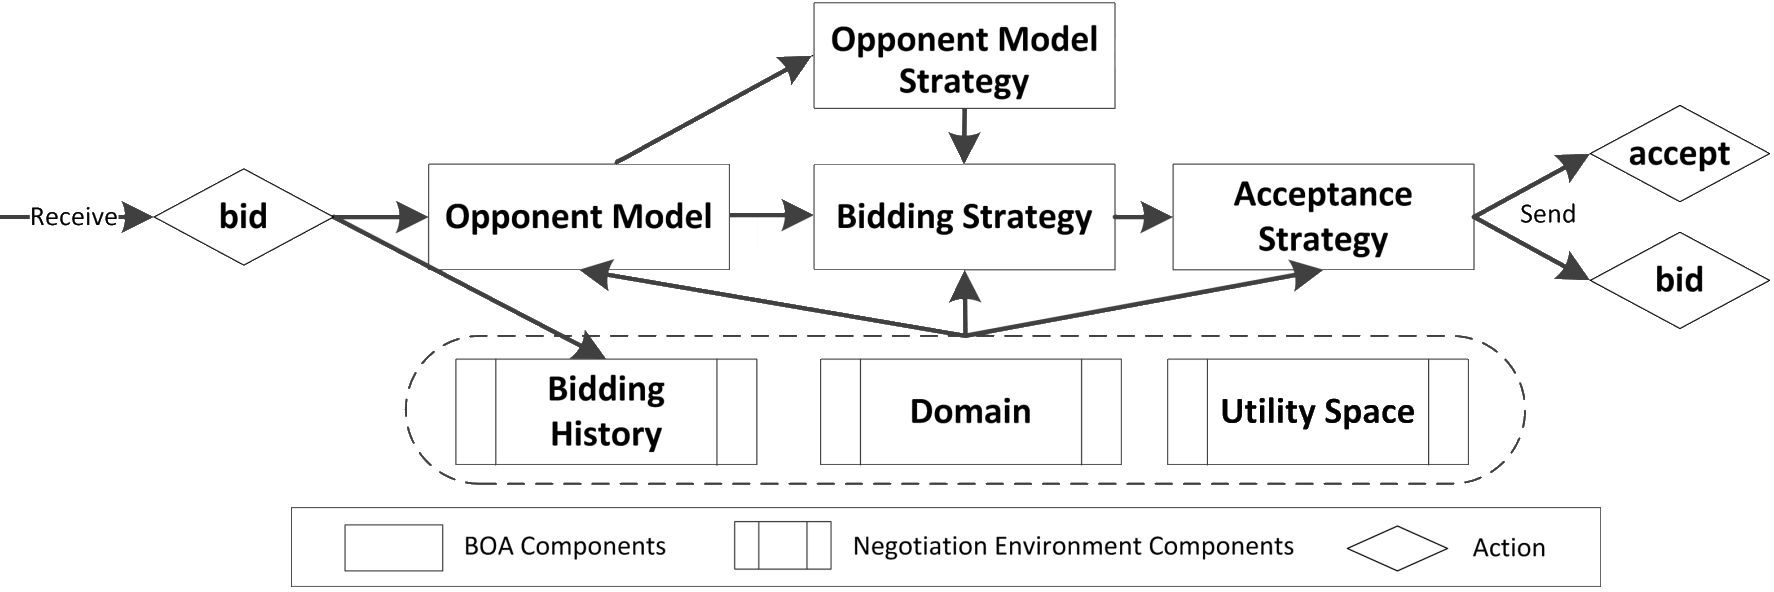
\includegraphics[width=15.0cm]{media/BOAflow.png}
	\caption{The BOA Framework Architecture.}
	\label{fig:flowchart}
\end{figure}
\pagebreak
\subsection{Using Existing Components}
In this section we create a \textit{BOA agent} by selecting its components from a list of existing components. The BOA framework GUI (see Figure~\ref{fig:decoupledGUI}) can be opened by double clicking the \textit{Values} section next to the \textit{BOA Agent side A} or \textit{BOA Agent side B} when creating a (distributed) tournament.

\begin{figure}[h!]
	\center
	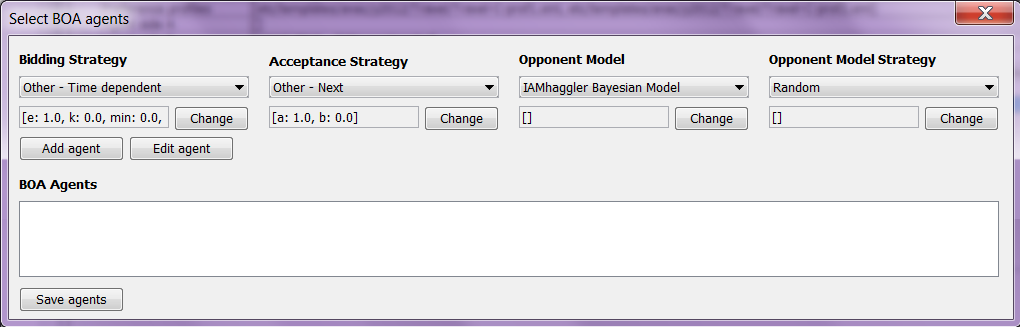
\includegraphics[width=15cm]{media/BOAgui.png}
	\caption{The BOA framework GUI.}
	\label{fig:decoupledGUI}
\end{figure}

Our goal in this section is to specify three BOA agents which are equal except for a single parameter $a$ of their acceptance strategy. 

To add the agents, click on the "Add agent(s)" button. A dialog pops up to enter the BOA agent details (Figure~\ref{fig:boadetails}).

\begin{figure}[h!]
	\center
	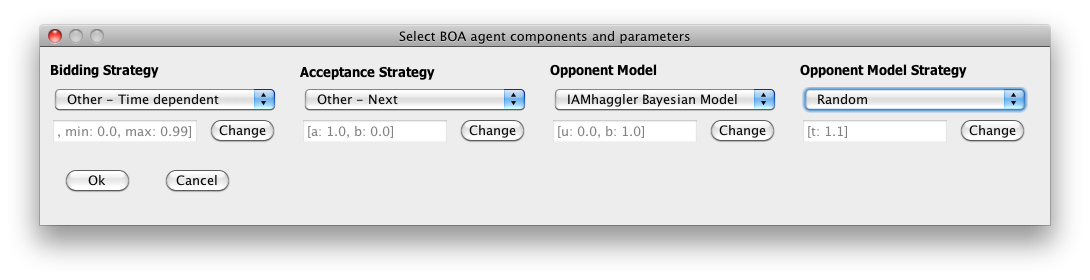
\includegraphics[width=15cm]{media/BOAdetails.png}
	\caption{The BOA agent components and parameters dialog.}
	\label{fig:boadetails}
\end{figure}

We select the bidding strategy \textit{Other - Time Dependent} under the heading \textit{Bidding Strategy}. Note that when we select this strategy, the default parameters of the component appear in the textbox below. Next, we select the other three components shown in Figure~\ref{fig:boadetails}.

The next step is to specify three variants of the acceptance strategy differing in the parameter $a$. To be more precise, we want $a$ to be 1.0, 1.1, and 1.2. To achieve this, press the ``Change'' button under  \textit{Acceptance Strategy}  to open a window similar to Figure~\ref{fig:boaparam}. Next, fill in the fields as shown in Figure~\ref{fig:boaparam}. Finally, we select ``Add agent(s)'' to create the three agents. Press "Save agents" to save the new BOA agents for the tournament. Note that in this example we only varied a single parameter of a single component. If we vary more parameters possibly of different components, then all possible combinations are generated.

\begin{figure}[h!] 
	\center
	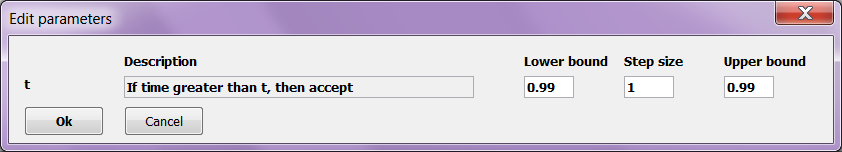
\includegraphics[width=15cm]{media/BOAparam.png}
	\caption{Adding a parameter.}
	\label{fig:boaparam}
\end{figure}

\subsection{Creating New Components}
This section discusses how create your own components. An example implementation of each component is included in the ``boaexamplepackage'' folder. The next section discusses how these components can be added to the list of available components in the BOA framework GUI.

\subsubsection{Parameters}
All BOA components have the same mechanism to be tuned with parameters. 

The parameters and their default parameters are indicated by the component by overriding the getParameters() function. This function should return a set of $BAOparameter$ objects, each parameter having a unique name, description and default value.


\begin{table}[h]
\begin{tabular}{m{0.9\textwidth}}
\hline
\texttt{public Set<BOAparameter> getParameters() }\\
 Override this function to add parameters to the module.\\
\hline
\end{tabular}
\caption{The getParameters method. Override if your component has parameters.}
\label{tab:parameters}
\end{table}


When the component is actually used, the actual values for the parameters (which may differ from the default) are passed to the init function when the component is initialized.

\subsubsection{Creating a Bidding Strategy}
A bidding strategy can be easily created by extending the \textit{OfferingStrategy} class. Table~\ref{tab:BOAbs} depicts the methods which need to be overridden. The \textit{init} method of the bidding strategy is automatically called by the BOA framework with four parameters: the negotiation session, the opponent model, the opponent model strategy, and the parameters of the component. The negotiation session object keeps track of the negotiation state, which includes all offers made by both agents, the timeline, the preference profile, and the domain. The parameters object specifies the parameters as specified in the GUI. In the previous section we specified the parameter $b$ for the acceptance strategy $Other - Next$ to be 0.0. In this case the agent can retrieve the value of the parameter by calling \textit{parameters.get(``b'')}.

An approach often taken by many bidding strategies is to first generate all possible bids. This can be efficiently done by using the \textit{SortedOutcomeSpace} class. For an example on using this class see the \textit{TimeDependent\_Offering} class in the \textit{boaexamplepackage} directory.

\begin{table}[h]
\begin{tabular}{m{0.9\textwidth}}
\hline
\texttt{void init(NegotiationSession negotiationSession, OpponentModel opponentModel, 
						OMStrategy omStrategy, HashMap<String, Double> parameters)}\\
Method directly called after creating the agent which should be used to initialize the component.\\
\hline
\texttt{BidDetails determineOpeningBid()}\\
Method which determines the first bid to be offered to the component.\\
\hline
\texttt{BidDetails determineNextBid()}\\
Method which determines the bids offered to the opponent after the first bid.\\
\hline
\end{tabular}
\caption{The main methods of the bidding strategy component.}
\label{tab:BOAbs}
\end{table}


\subsubsection{Creating an Acceptance Condition}
This section discusses how to create an acceptance strategy class by extending the abstract class \textit{AcceptanceStrategy}. Table~\ref{tab:BOAas} depicts the two methods which need to specified.

\begin{table}[h]
\begin{tabular}{m{0.9\textwidth}}
\hline
\texttt{void init(NegotiationSession negotiationSession, OfferingStrategy offeringStrategy,
						OpponentModel opponentModel, HashMap<String, Double> parameters)}\\
Method directly called after creating the agent which should be used to initialize the component.\\
\hline
\texttt{Actions determineAcceptability()}\\
Method which determines if the agent should accept the opponent's bid (\textit{Actions.Accept}), reject it and send a counter offer (\textit{Actions.Reject}), or leave the negotiation (\textit{Actions.Break}).\\
\hline
\end{tabular}
\caption{The main methods of the acceptance strategy component.}
\label{tab:BOAas}
\end{table}

\subsubsection{Creating an Opponent Model}
This section discusses how to create an opponent model by extending the abstract class \textit{OpponentModel}. Table~\ref{tab:BOAom} provides an overview of the main methods which need to specified. For performance reasons it is recommended to use the \textit{UtilitySpace} class.

\begin{table}[h]
\begin{tabular}{m{0.9\textwidth}}
\hline
\texttt{void init(NegotiationSession negotiationSession, HashMap<String, Double> parameters)}\\
Method directly called after creating the agent which should be used to initialize the component.\\
\hline
\texttt{double getBidEvaluation(Bid bid)}\\
Returns the estimated utility of the given bid.\\
\hline
\texttt{double updateModel(Bid bid)}\\
Updates the opponent model using the given bid.\\
\hline
\texttt{UtilitySpace getOpponentUtilitySpace()}\\
Returns the opponent's preference profile. Use the \textit{UtilitySpaceAdapter} class when not using the UtilitySpace class for the opponent's preference profile.\\
\hline
\end{tabular}
\caption{The main methods of the opponent model component.}
\label{tab:BOAom}
\end{table}

\subsubsection{Creating an Opponent Model Strategy}
This section discusses how to create an opponent model strategy by extending the abstract class \textit{OMStrategy}. Table~\ref{tab:BOAoms} provides an overview of the main methods which need to specified.

\begin{table}[h]
\begin{tabular}{m{0.9\textwidth}}
\hline
\texttt{void init(NegotiationSession negotiationSession, OpponentModel model, HashMap<String, Double> parameters)}\\
Method directly called after creating the agent which should be used to initialize the component.\\
\hline
\texttt{BidDetails getBid(List<BidDetails> bidsInRange);}\\
This method returns a bid to be offered from a set of given similarly preferred bids by using the opponent model.\\
\hline
\texttt{boolean canUpdateOM();}\\
Determines if the opponent model may be updated this turn.\\
\hline
\end{tabular}
\caption{The main methods of the opponent model strategy component.}
\label{tab:BOAoms}
\end{table}

\subsection{Compiling BOA Components}
BOA components must be compiled before they can be loaded into Genius.
To compile a BOA component, do the following steps (in this example we compile the boa example components)
\begin{itemize}
\item Open a terminal 
\item Switch to the root directory of genius
\item Enter the command \texttt{javac -cp negosimulator.jar -source 1.6 -target 1.6 boaexamplepackage/*.java }
\end{itemize}

You can also compile from Eclipse or Netbeans. Make sure you add the negosimulator.jar to your class path. Please refer to the Eclipse or Netbeans documentation on how to do this.


\subsection{Adding a Component to the BOA Repository}
In the previous section we discussed how to create each type of BOA component. To use the components, we still need to add them to the \textit{BOA repository}. To do so, open the BOA components tab in the components window as shown in Figure~\ref{fig:boacomponents}. Right click and select ``Add new component''. This results in the opening of the window shown in Figure~\ref{fig:loadBOA}.

\begin{figure}[h!] 
	\center
	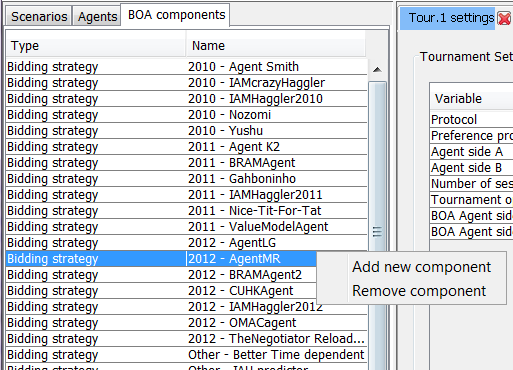
\includegraphics[width=7cm]{media/AddBOA.png}
	\caption{The BOA components window.}
	\label{fig:boacomponents}
\end{figure}

Click on the "Open" button and select the main class file of your BOA component (the class file that implements the BOA interface). Then check the name of the component, you can change it but it has to be a unique name in the registry. Optionally add parameters. Finally, clicking ``Add component'' in this window adds the component to the repository.

\begin{figure}[h!] 
	\center
	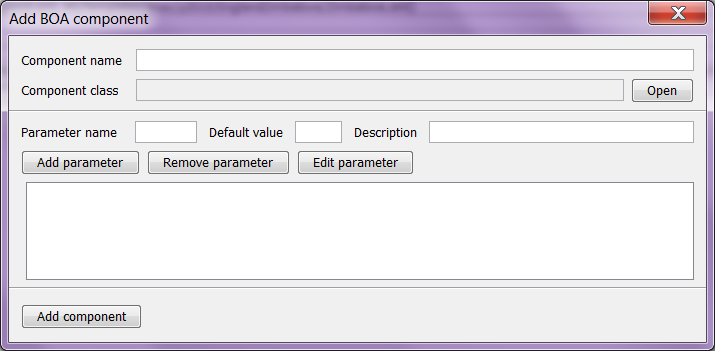
\includegraphics[width=5cm]{media/LoadBOA.png}
	\caption{Loading a BOA agent.}
	\label{fig:loadBOA}
\end{figure}


\subsection{Creating a ANAC2013 BOA Agent}\label{sec:anac2013agentBOA}
In Section~\ref{sec:anac2013agent} we discussed how to create an agent for the ANAC2013. Using a similar procedure it is also possible to create BOA agents compatible with ANAC2013. An example to do so is included in this distribution of \Genius.

As only a single object can be saved and loaded, the BOA framework stores an object \textit{SessionData} that includes the data saved by all three components. This object is loaded and saved automatically by the BOA framework. A component can easily access the data it saved by using the \textit{loadData} method. A component can at each moment during the negotiation update the saved information by using the \textit{storeData} method, although we recommend updating the information at the end of the negotiation by using the the \textit{endSession} method. The \textit{endSession} method of each method is automatically called at the end of the negotiation to inform the component of the result obtained and should be used to update the \textit{SessionData} object before it is automatically stored.

\subsection{Advanced: Converting a BOA Agent to an Agent}
To convert a BOA agent to a normal agent you have to create a class that extends \textit{BOA agent} and override the \textit{agentSetup} method. Below is an example of a BOA agent wrapped as a normal agent.

\begin{lstlisting}
public class SimpleBOAagent extends BOAagent{

	@Override
	public void agentSetup() {
		OpponentModel om = new FrequencyModel(negotiationSession, 0.2, 1);
		OMStrategy oms = new NullStrategy(negotiationSession);
		OfferingStrategy offering  = new TimeDependent_Offering(negotiationSession,
								om, oms, 0.2, 0, 1, 0);
		AcceptanceStrategy ac = new AC_Next(negotiationSession, offering, 1, 0);
		setDecoupledComponents(ac, offering, om, oms);		
	}

	@Override
	public String getName() {
		return "SimpleBOAagent";
	}
}
\end{lstlisting}

\subsection{Advanced: Multi-Acceptance Criteria (MAC)}
The \textit{BOA framework} allows us to better explore a large space of negotiation strategies. MAC can be used to scale down the negotiation space, and thereby make it better computationally explorable.

As discussed in the introduction of this chapter, the acceptance condition determines solely if a bid should be accepted. This entails that it does not influence the bidding trace, except for when it is stopped. In fact, the only difference between \textit{BOA agents} where only the acceptance condition vary, is the time of agreement (assuming that the computational cost of the acceptance conditions are negligible).

Given this property, multiple acceptance criteria can be tested in parallel during the same negotiation trace. In practice, more than 50 variants of a simple acceptance condition as for example $\textbf{AC}_{next}$ can be tested in the same negotiation at a negligible computational cost.

To create a multi-acceptance condition component you first need to extend the class \textit{Mulit Acceptance Condition}, this gives access to the ACList which is a list of acceptance conditions to be tested in parallel. Furthermore, the method \textit{isMac} should be overwritten to return \textit{true} and the name of the components in the repository should be \textit{Multi Acceptance Criteria}. An acceptance can be added to the MAC by appending it to the AClist as sown below. 

\begin{lstlisting}
public class AC_MAC extends Multi_AcceptanceCondition {
	@Override
	public void init(NegotiationSession negoSession, OfferingStrategy strat, 
			OpponentModel opponentModel, HashMap<String, Double> parameters)
			throws Exception {
		this.negotiationSession = negoSession;
		this.offeringStrategy = strat;
		outcomes = new ArrayList<OutcomeTuple> ();
		ACList = new ArrayList<AcceptanceStrategy>();
		for (int e = 0; e < 5; e++) {
			ACList.add(new AC_Next(negotiationSession, offeringStrategy, 1, 
												e * 0.01));
		}
	}
}

\end{lstlisting}




%=========================================================================================

\section{Creating a Multi Party Negotiation Agent}
This section discusses how to create a multilateral negotiation agent in Java. Multilateral means you can use this agent in a multi-party negotation and multi-party tournament but not in a two-party negotiation or tournament. Notice that you can still do two-party negotiations in the multilateral negotiation and tournament.

To implement a multi-party negotiation party, at a minimum one needs to implement a class that implements the \\texttt{negotiator.parties.NegotiationParty} interface. Also this class must have a public default (no-argument) constructor.
To implement the interface, one needs to implement five functions: 

\begin{lstlisting}
public interface NegotiationParty {
	/**
	 * This is the first call made to a NegotiationParty after its
	 * instantiation. Tells which utility space and timeline we are running in.
	 * This is called one time only.
	 *
	 * @param utilSpace
	 *            (a copy of/readonly version of) the {@link UtilitySpace} to be
	 *            used for this session.
	 * @param timeline
	 *            The {@link TimeLineInfo} about current session.
	 * @param agentID
	 *            the {@link AgentID}.
	 * @throws RuntimeException
	 *             if init fails.
	 */
	public void init(UtilitySpace utilSpace, Deadline deadline,
			TimeLineInfo timeline, long randomSeed, AgentID agentID);

	/**
	 * When this function is called, it is expected that the Party chooses one
	 * of the actions from the possible action list and returns an instance of
	 * the chosen action.
	 *
	 * @param possibleActions
	 *            List of all actions possible.
	 * @return The chosen {@link Action}.
	 */
	public Action chooseAction(List<Class<? extends Action>> possibleActions);

	/**
	 * This method is called when another {@link NegotiationParty} chose an
	 * {@link Action}.
	 *
	 * @param sender
	 *            The initiator of the action. May be null if initiator is not an agent.
	 * @param arguments
	 *            The action performed
	 */
	void receiveMessage(AgentID sender, Action arguments);

	/**
	 * @return a description for this party
	 */
	public String getDescription();

	/**
	 * Get the protocol that this party supports.
	 * 
	 * @return the actual supported {@link MultilateralProtocol}, usually
	 *         {@link StackedAlternatingOffersProtocol}.
	 */
	public Class<? extends MultilateralProtocol> getProtocol();

}
\end{lstlisting}

We recommend to use the javadoc included with the distribution to check the details of all the involved classes. 

But in practice, it may be more convenient to extend the class \texttt{negotiator.parties.AbstractNegotiationParty} that provides convenient support functions. 

The functions \verb|receiveMessage| and \verb|chooseAction| are basically the same as described in section \ref{sec:receiveAction} and \ref{sec:chooseAction}. getProtocol usually returns an instance of StackedAlternatingOffersProtocol.


\subsection{Compiling a NegotiationParty}


To compile the example agent, go to your genius project folder and use the command line to execute this compile command

\verb|javac -cp negosimulator.jar -source 1.6 -target 1.6  multipartyexample/Groupn.java|

\subsection{Loading a NegotiationParty}

You need to load your custom party into the party repository in order to use it. After adding, your agent will appear in the combo boxes in the multilateral tournament runner and session runner where you can select the party to use.

You can load the new NegotiationParty into the party repository in two ways:
\subsubsection{loading with the GUI}
Locate the Parties repository tab in the GUI (Figure \ref{fig:partiesrepo}). Right click in this area and select "Add Party". A browser window pops up. Brows to  your compiled class file that implements the NegotiationParty and select it. Your party will appear at the bottom of the parties repository. The partyrepository.xml file is automatically updated accordingly.

\begin{figure}[h!] 
	\center
	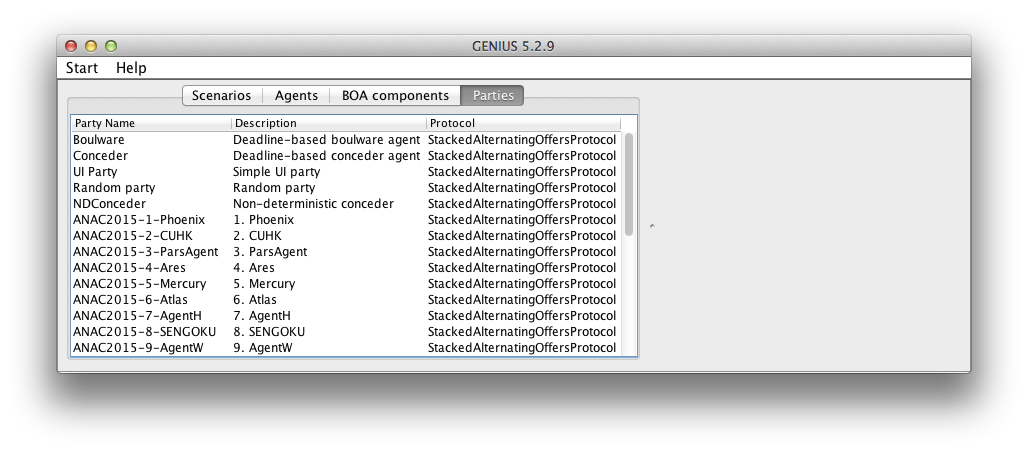
\includegraphics[width=10cm]{media/partiesrepo.png}
	\caption{The parties repository.}
	\label{fig:partiesrepo}
\end{figure}

\subsubsection{manual loading}
To do this manually, quit \Genius , open the \verb|partyrepository.xml| file and add a section like this

\begin{lstlisting}
<partyRepItem description="description for your agent"
	classPath="class.of.your.agent" partyName="nameForYourAgent"
	protocolClassPath="negotiator.protocol.StackedAlternatingOffersProtocol"/>
\end{lstlisting}

After that you can restart \Genius .

\section{Conclusion}
This concludes the manual of \Genius. If you experience problems or have suggestions on how to improve \Genius, please send them to \url{negotiation@ii.tudelft.nl}. 

\Genius\ is actively used in academic research. If you want to cite \Genius\ in your paper, please refer to \cite{Genius}.


\bibliographystyle{plain}
\bibliography{genius}

\end{document}